\chapter{Julia-Mengen}
\rhead{Julia-Mengen}
\begin{refsection}

\chapterauthor{Andreas M"uller}
\section{Was sind Julia-Mengen?}
F"ur jede komplexe Zahl $c\in\mathbb C$ kann man die Iterationen der
Funktion
\begin{equation}
f_c(z)=z^2 + c
\label{julia:quadratic}
\end{equation}
untersuchen.
Ausgehend von einem Anfangswert $z_0\in\mathbb C$ bilden wir die Folge
\[
z_1=f(z_0),\;z_2=f(z_1),\;z_3=f(z_2)\;\dots, z_{n+1}=f(z_n),\;\dots
\]
F"ur $|z|\ge |c|$ und $|z|\ge 3$ folgt
\[
|f_c(z)|= |z^2+c|\ge |z|^2-|c|\ge |z|^2-|z|=|z|(|z|-1)\ge |z|\ge 2|z|.
\]
Die Iterierten von $z_n$ wachsen exponentiell schnell "uber alle Grenzen.

Es ist aber auch m"oglich, dass f"ur einzelne Punkte die Folge $z_n$ 
gegen $\hat z$ konvergiert.
Der Punkt $\hat z$ ist ein Fixpunkt von $f_c$, denn
\[
\hat z = \lim_{n\to \infty}f_c^{n}(z)\quad\Rightarrow\quad
f_c(\hat z)=f_c(\lim_{n\to\infty}f_c^n(z))=\lim_{n\to\infty}f_c^{n+1}(z)=\hat z.
\]
Die Folge $z_n$ muss aber nicht unbedingt gegen einen Punkt konvergieren,
es kann auch einen Zyklus von $k$ Punkten $\hat z_1,\dots,\hat z_k$ geben
so, dass
\[
z_{kn+1}\to \hat z_1,\quad
z_{kn+2}\to \hat z_2,\quad
z_{kn+3}\to \hat z_3,\quad\dots,\quad
z_{kn+k}\to \hat z_k.
\]
Die komplexe Ebene besteht also aus h"ochstens zwei Regionen: dem Bereich
von komplexen Zahlen, die bei Iteration "uber alle Grenzen wachsen, und
einem Bereich von Punkten, die bei Iteration gegen einen Zyklus konvergieren.
Die Grenze zwischen den beiden Bereichen besteht aus Punkten, die weder gegen
$\infty$ noch gegen $\hat z$ konvergieren. Diese Grenze heisst die Julia-Menge
von $f_c$.

\begin{beispiel}
Im Fall $c=0$ ist $f_0(z)=z^2$. Da jede komplexe Zahl geschrieben werden
kann als $z=re^{i\varphi}$, sind die Iterierten von $f_0$:
\[
z_1=r^2e^{2i\varphi},
z_2=r^4e^{4i\varphi},
z_3=r^8e^{8i\varphi},
z_4=r^{16}e^{16i\varphi},\dots,
z_n=r^{2^n}e^{2^ni\varphi},\dots
\]
Wenn $r < 1$ ist, dann werden die Iterierten $z_n$ immer kleiner, die
Folge konvergiert gegen $0$.
Falls $r>1$ dann wachsen die Iterierten "uber alle Grenzen.
Im Falle $r=1$ bleiben die Iterierten auf dem Einheitskreis.
Die komplexe Ebene wird also in drei Bereiche geteilt: das
Innere des Einheitskreises besteht aus Zahlen, deren Iterierte gegen
0 konvergieren, das "Aussere des Einheitskreises besteht aus Zahlen,
deren Iterierte gegen $\infty$ konvergieren.
Die Grenze zwischen den beiden Bereichen ist der Einheitskreis selber,
die Iterierten der Zahlen auf dem Einheitskreis konvergieren im
allgemeinen nicht.

Der Einheitskreis ist die Julia-Menge der Abbildung $f_c$ f"ur $c=0$.
\end{beispiel}

F"ur andere Werte des Parameters kann die Julia-Menge sehr kompliziert
werden, so kompliziert, dass sie nur dank Computer-Berechnungen
ausreichend detailliert visualisiert werden kann.

Die Iteration der quadratischen Abbildungen (\ref{julia:quadratic})
wurden sorgf"altig studiert, sie sind relativ einfach, zeigen aber
trotzdem viele Eigenschaften der nichtlinearen dynamischen Systeme.
Insbesondere zeigt schon $f_0$ auf dem Einheitskreis chaotisches
Verhalten \cite{julia:devaney}.

Die Julia-Mengen werden derart kompliziert, dass man ihnen keine ganzzahlige
Dimension mehr zuweisen kann. Vergr"ossert man einen Ausschnitt, werden
immer mehr Details sichtbar, die ``Kurve'' wird immer komplizierter.
Ist ist oft m"oglich, den Julia-Mengen eine gebrochenzahlen Dimension
zuzuweisen.
Die Definition dieser gebrochenzahligen Dimensionen ist nicht ganz
selbstverst"andlich, Mengen mit gebrochenzahliger Dimension treten
aber mindestens n"aherungsweise in der Natur immer wieder auf, sie
sind auch als Fraktale bekannt \cite{julia:falconer}.

\section{Berechnung von Julia-Mengen}
Es gibt zwei M"oglichkeiten, eine Julia-Menge sichtbar zu machen.
In den F"allen, wo ein Fixpunkt $\hat z$ existiert, kann man f"ur jeden
Punkt der komplexen Ebene die Iterationsfolge $z_n$ berechnen, und
entscheiden ob sie gegen $\infty$ oder einen Zyklus konvergiert.
Die Juliamenge ist dann die Grenze zwischen diesen Bereichen.

Dies funktioniert allerdings nicht f"ur Parameterwerte, f"ur die
es keinen Zykles gibt, gegen den die Folge $z_n$ konvergieren k"onnte.
In diesem Fall kann man die Abbildung $f_c(z)$ umkehren: wenn die
Punkte $z_n$ von der Julia-Menge weg gegen $\infty$ konvergieren, dann 
m"ussen die Urbilder gegen die Juliamenge konvergieren.
Man kann also die Julia-Menge dadurch finden, dass man alle Urbilder
bestimmt.

\subsection{Julia-Mengen durch Iteration}
Um ein Bild der Julia-Menge zum Parameter $c$ zu erhalten, berechnet
man f"ur jeden Startpunkt $z_0\in\mathbb C$ die Folge $z_n$ und
bestimmt den kleinsten Wert $n$, f"ur den $|z_n|>b$ ist, wobei $b$
irgend eine fest Schranke ist.
Der Pixel zum Punkt $z_0$ wird mit einer Farbe eingef"arbt, die von $n$
abh"angt.
Falls $z_n$ die Grenze $b$ nicht "uberschreitet, bleibt der Pixel schwarz.

Die Berechnung der Iterationsfolge ist f"ur jeden Pixel vollkommen
unabh"angig von jedem anderen Pixel, dieses Beispiel ist als pr"adestiniert
f"ur die Berechnung mit OpenCL.
Jeder Pixel stellt ein eigenes Work-Item dar.
Das Programm {\tt julia.c} im Repository implementiert diese Strategie.


\subsection{Julia-Mengen durch Inverse Iteration}
Jeder Punkt $z\in\mathbb C$ hat zwei Urbilder unter der Abbildung $f_c$,
denn
\[
z=f_c(\tilde z)=\tilde z^2+c
\qquad\Rightarrow\qquad
\tilde z=\sqrt{z-c}
\]
hat zwei Quadratwurzeln. 
Die zwei Urbilder von $z$ haben unter $f_c$ insgesamt vier Urbilder, 
die wiederum acht Urbilder.
Jede weitere Iteration verdoppelt die Anzahl der Urbilder, daf"ur ist
in OpenCL kein Platz vorhanden.

Wir verwenden daher eine andere Strategie: wir w"ahlen jeweils nur eines
der Urbilder, wobei wir Zufallszahlen verwenden, um eines der zwei
Urbilder zu w"ahlen.
Diese Berechnung wiederholen wir viele Male, jeweils mit einer anderen
Zufallszahlfolge.
Auf diese Weise werden ebenfalls alle Punkte der Julia-Menge irgendwann
approximiert.

Mit dieser Strategie handeln wir uns aber ein neues Problem ein, wir brauchen
eine Folge von Zufallszahlen.
OpenCL stellt kein API f"ur Zufallszahlen zur Verf"ugung, dies muss also
ebenfalls im OpenCL Code implementiert werden.
Die Anforderungen an die Qualit"at der Zufallszahlen ist nicht besonders
hoch, ein einfacher Zufallszahlgenerator auf der Basis von linearen
Kongruenzen wie der Lehmer-Generator \cite{julia:lehmer},
auch bekannt als Park-Miller Generator, reicht v"ollig aus.

\begin{figure}
\begin{center}
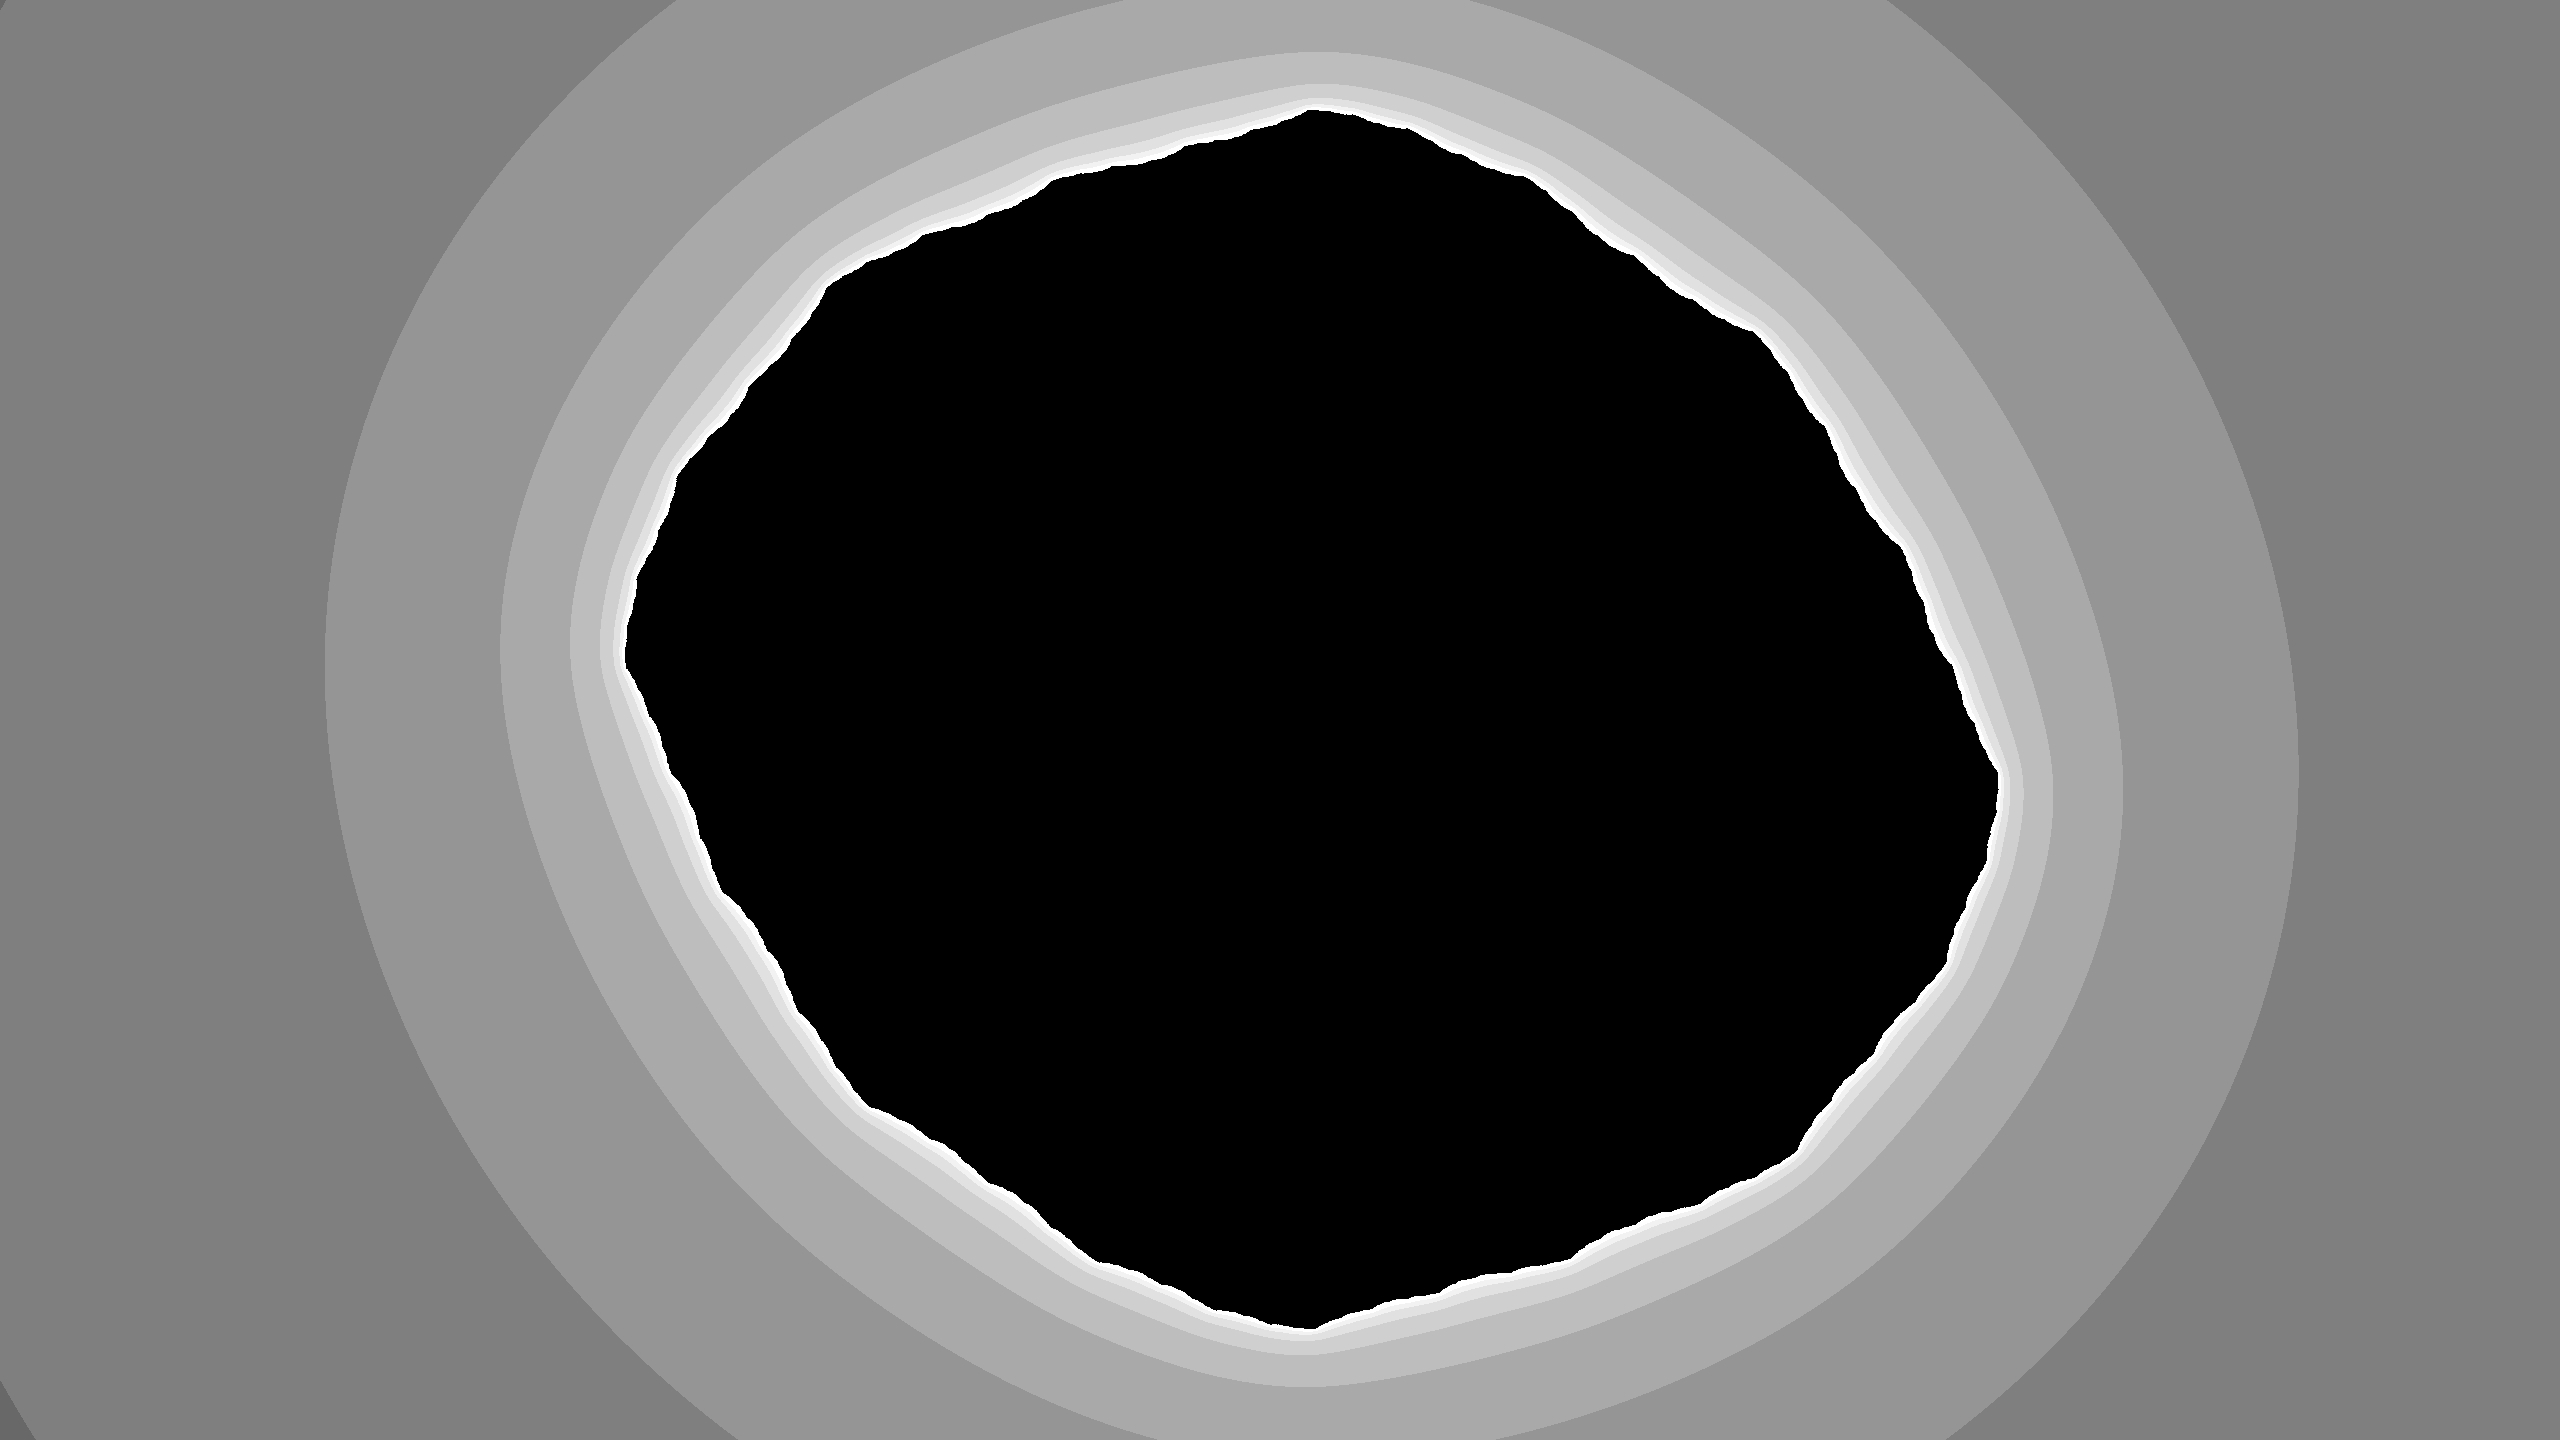
\includegraphics[width=\hsize]{julia/a.png}

\bigskip

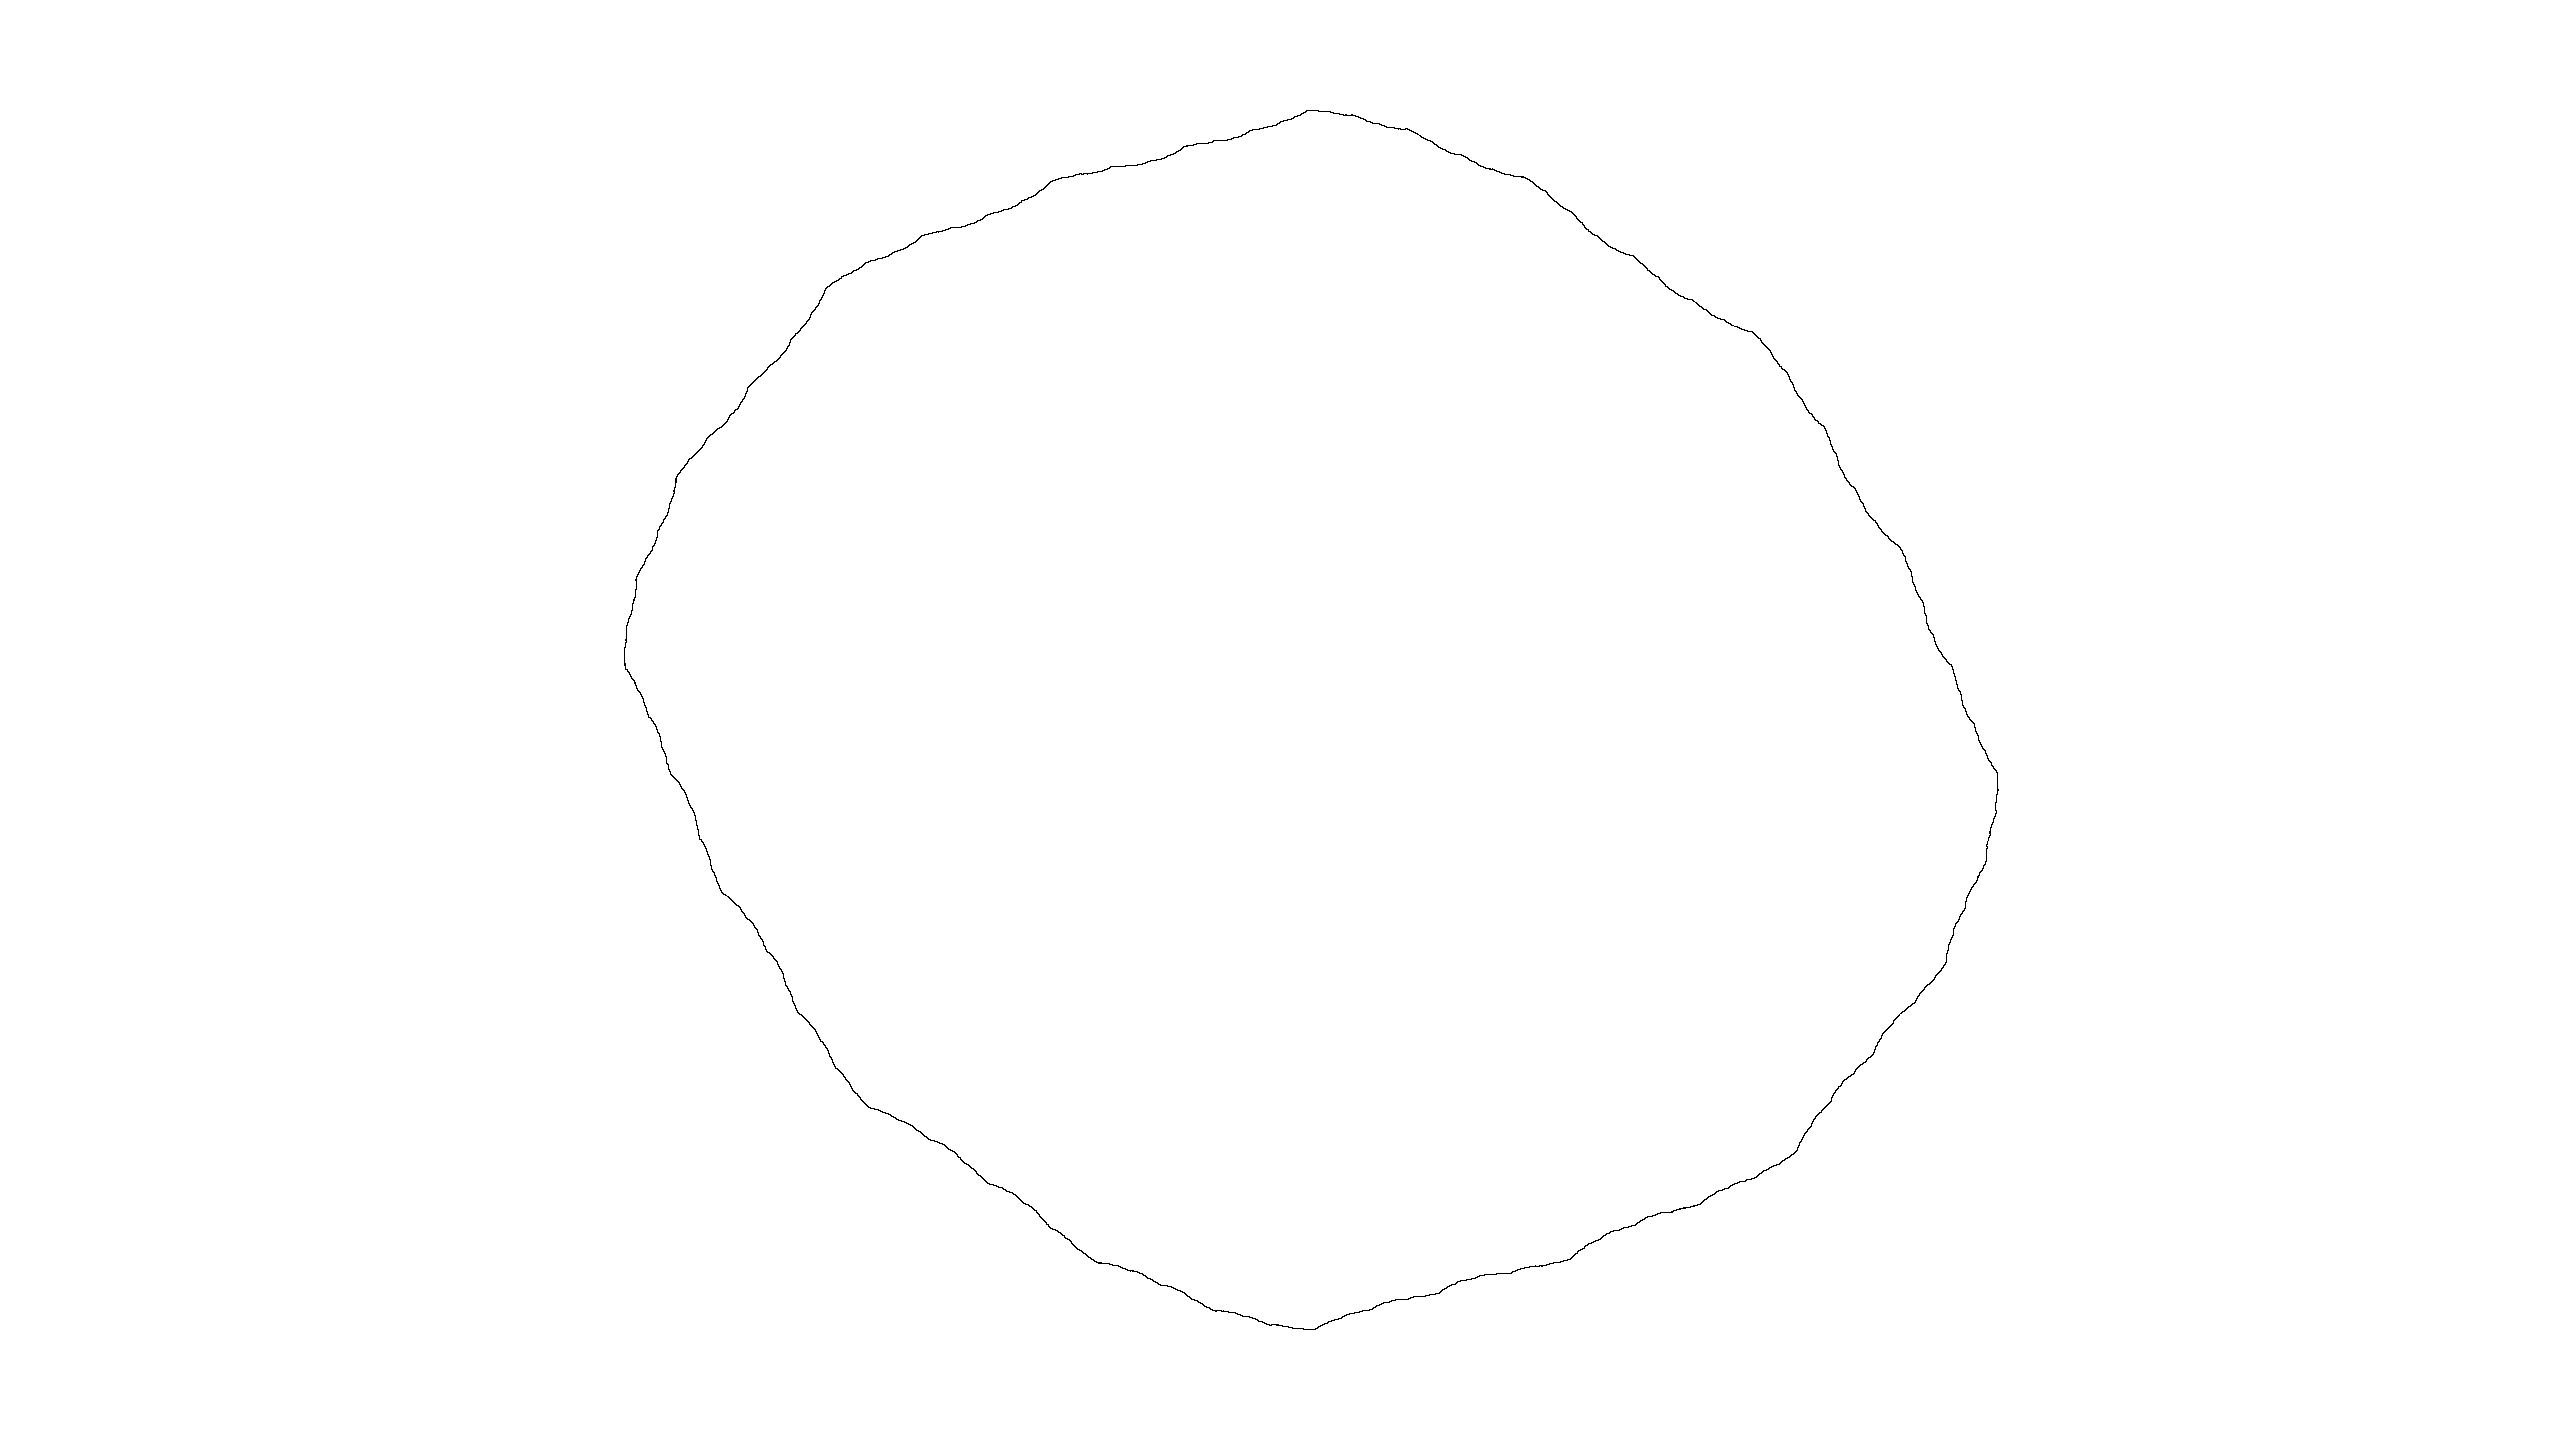
\includegraphics[width=\hsize]{julia/j-a.png}
\end{center}
\caption{Julia-Menge f"ur $c= -0.1+0.1i$}
\end{figure}

\begin{figure}
\begin{center}
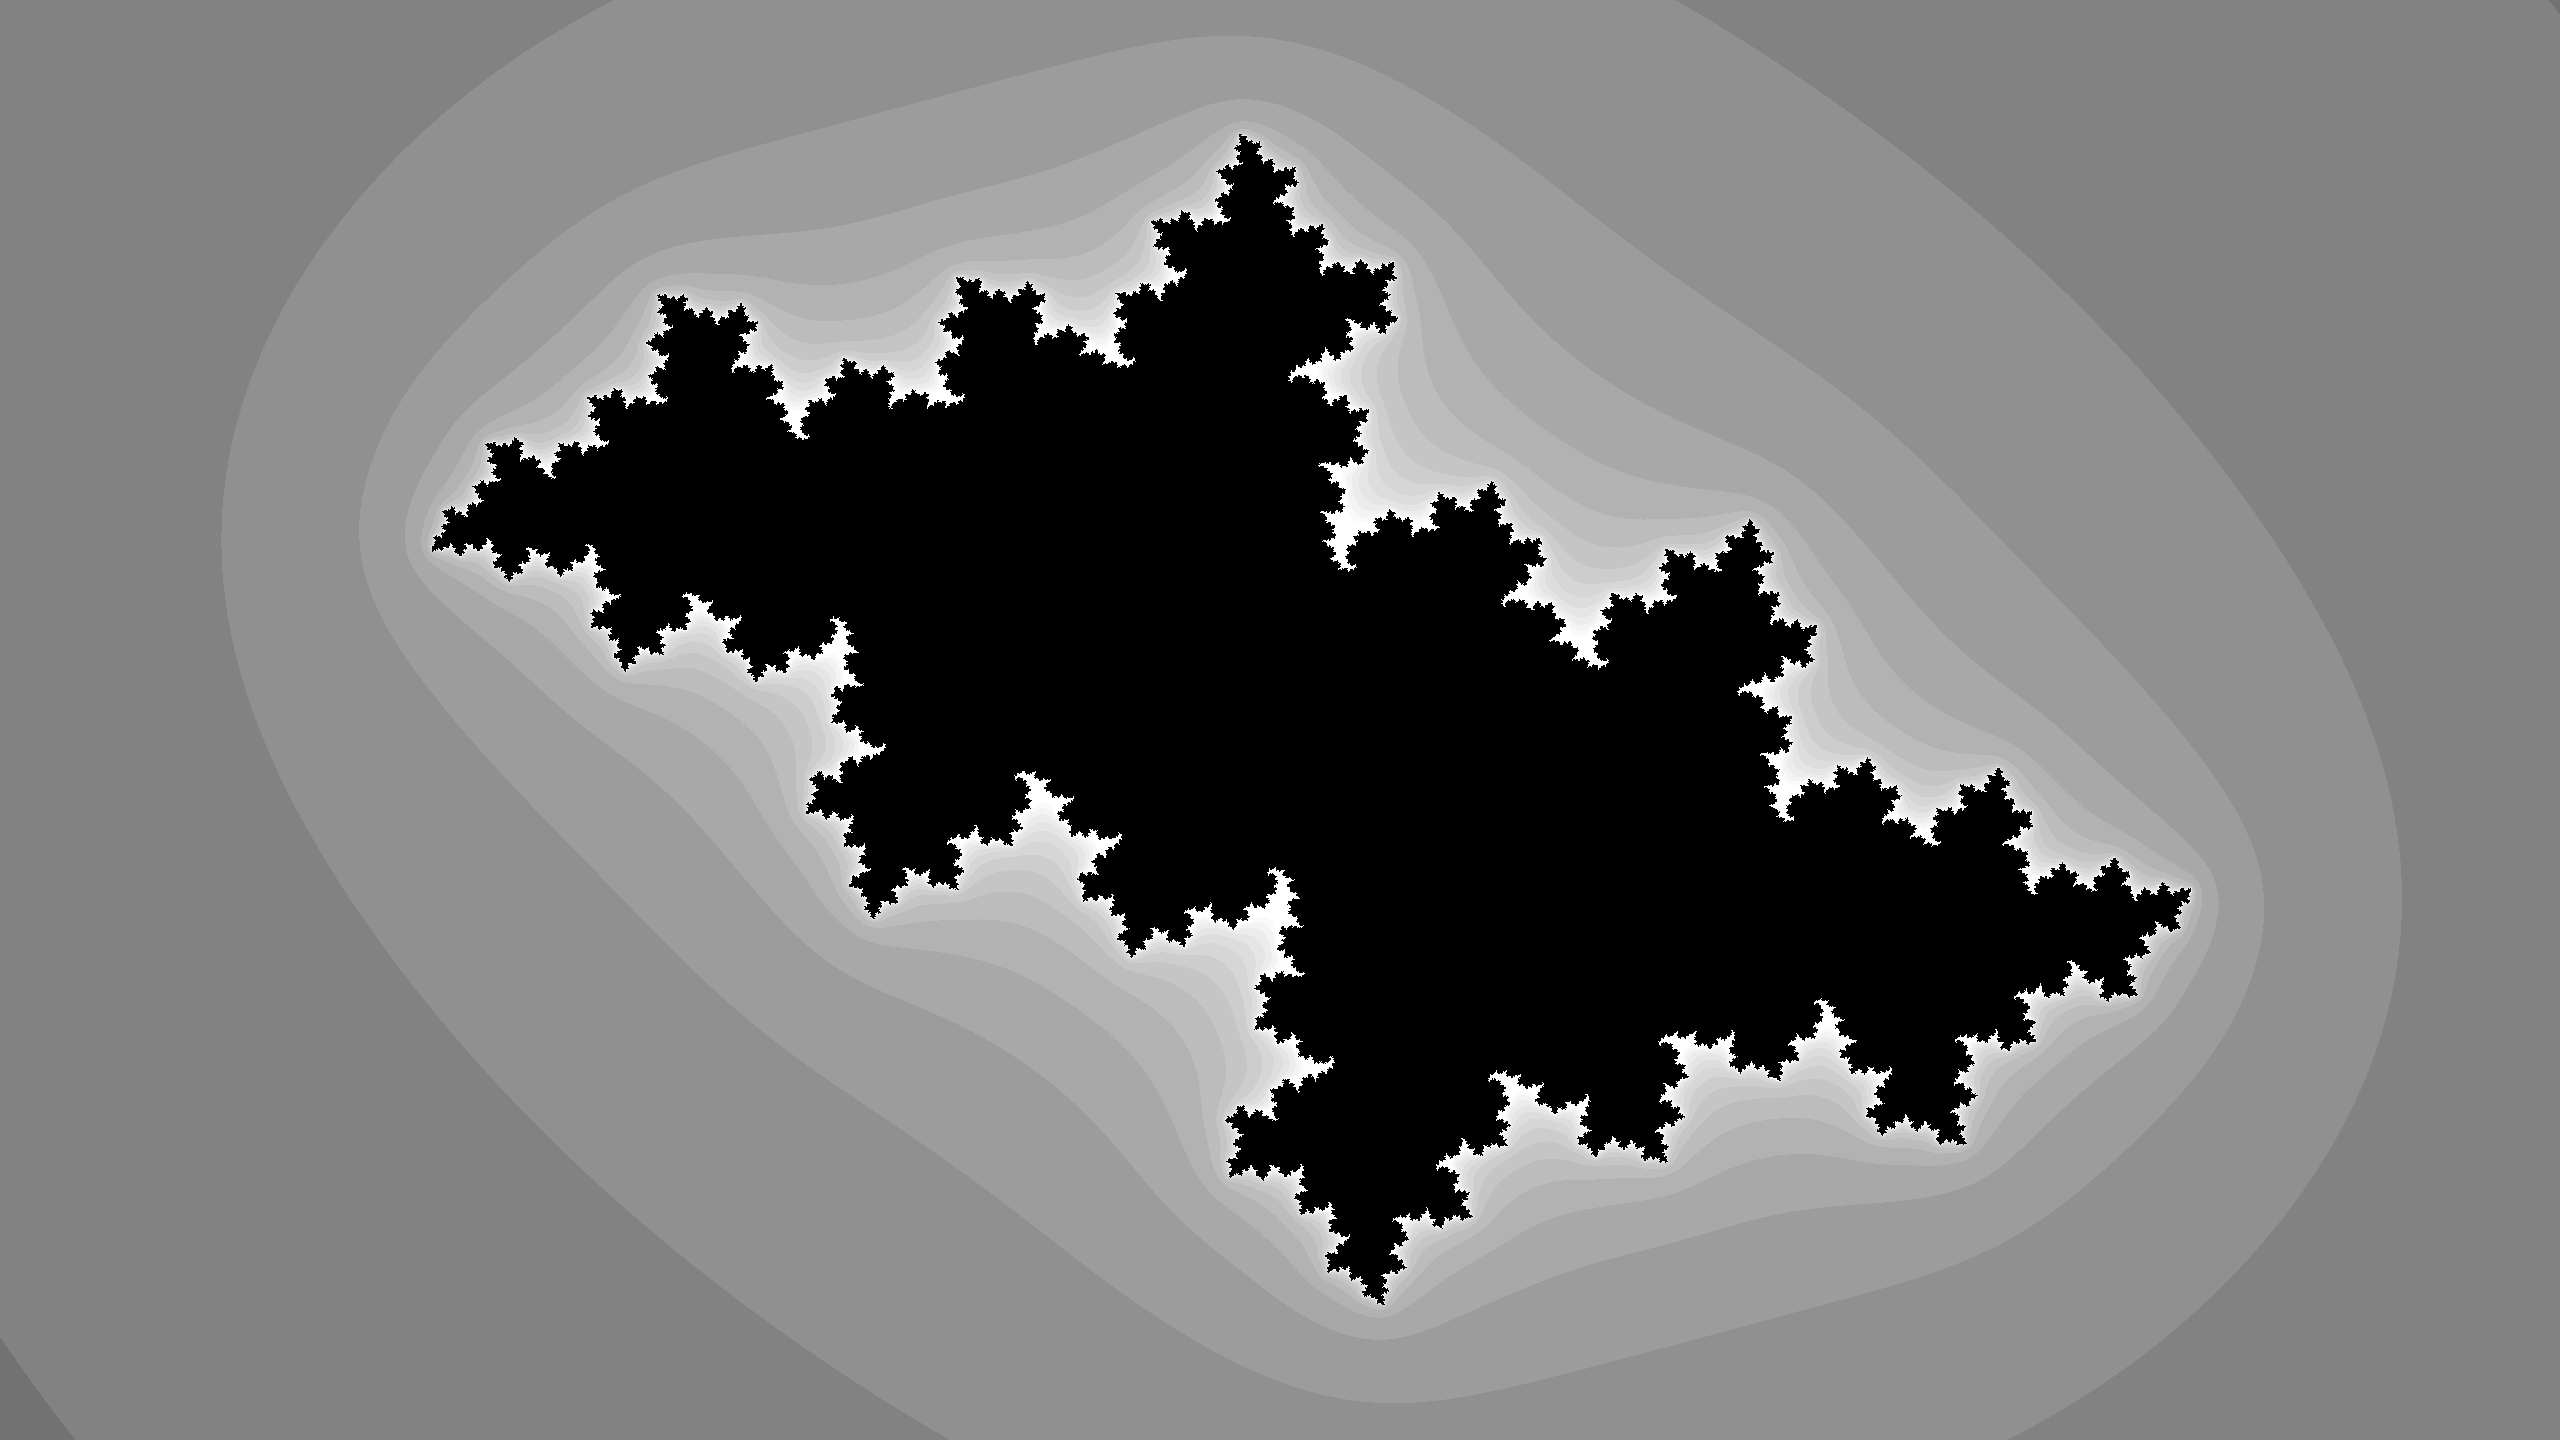
\includegraphics[width=\hsize]{julia/b.png}

\bigskip

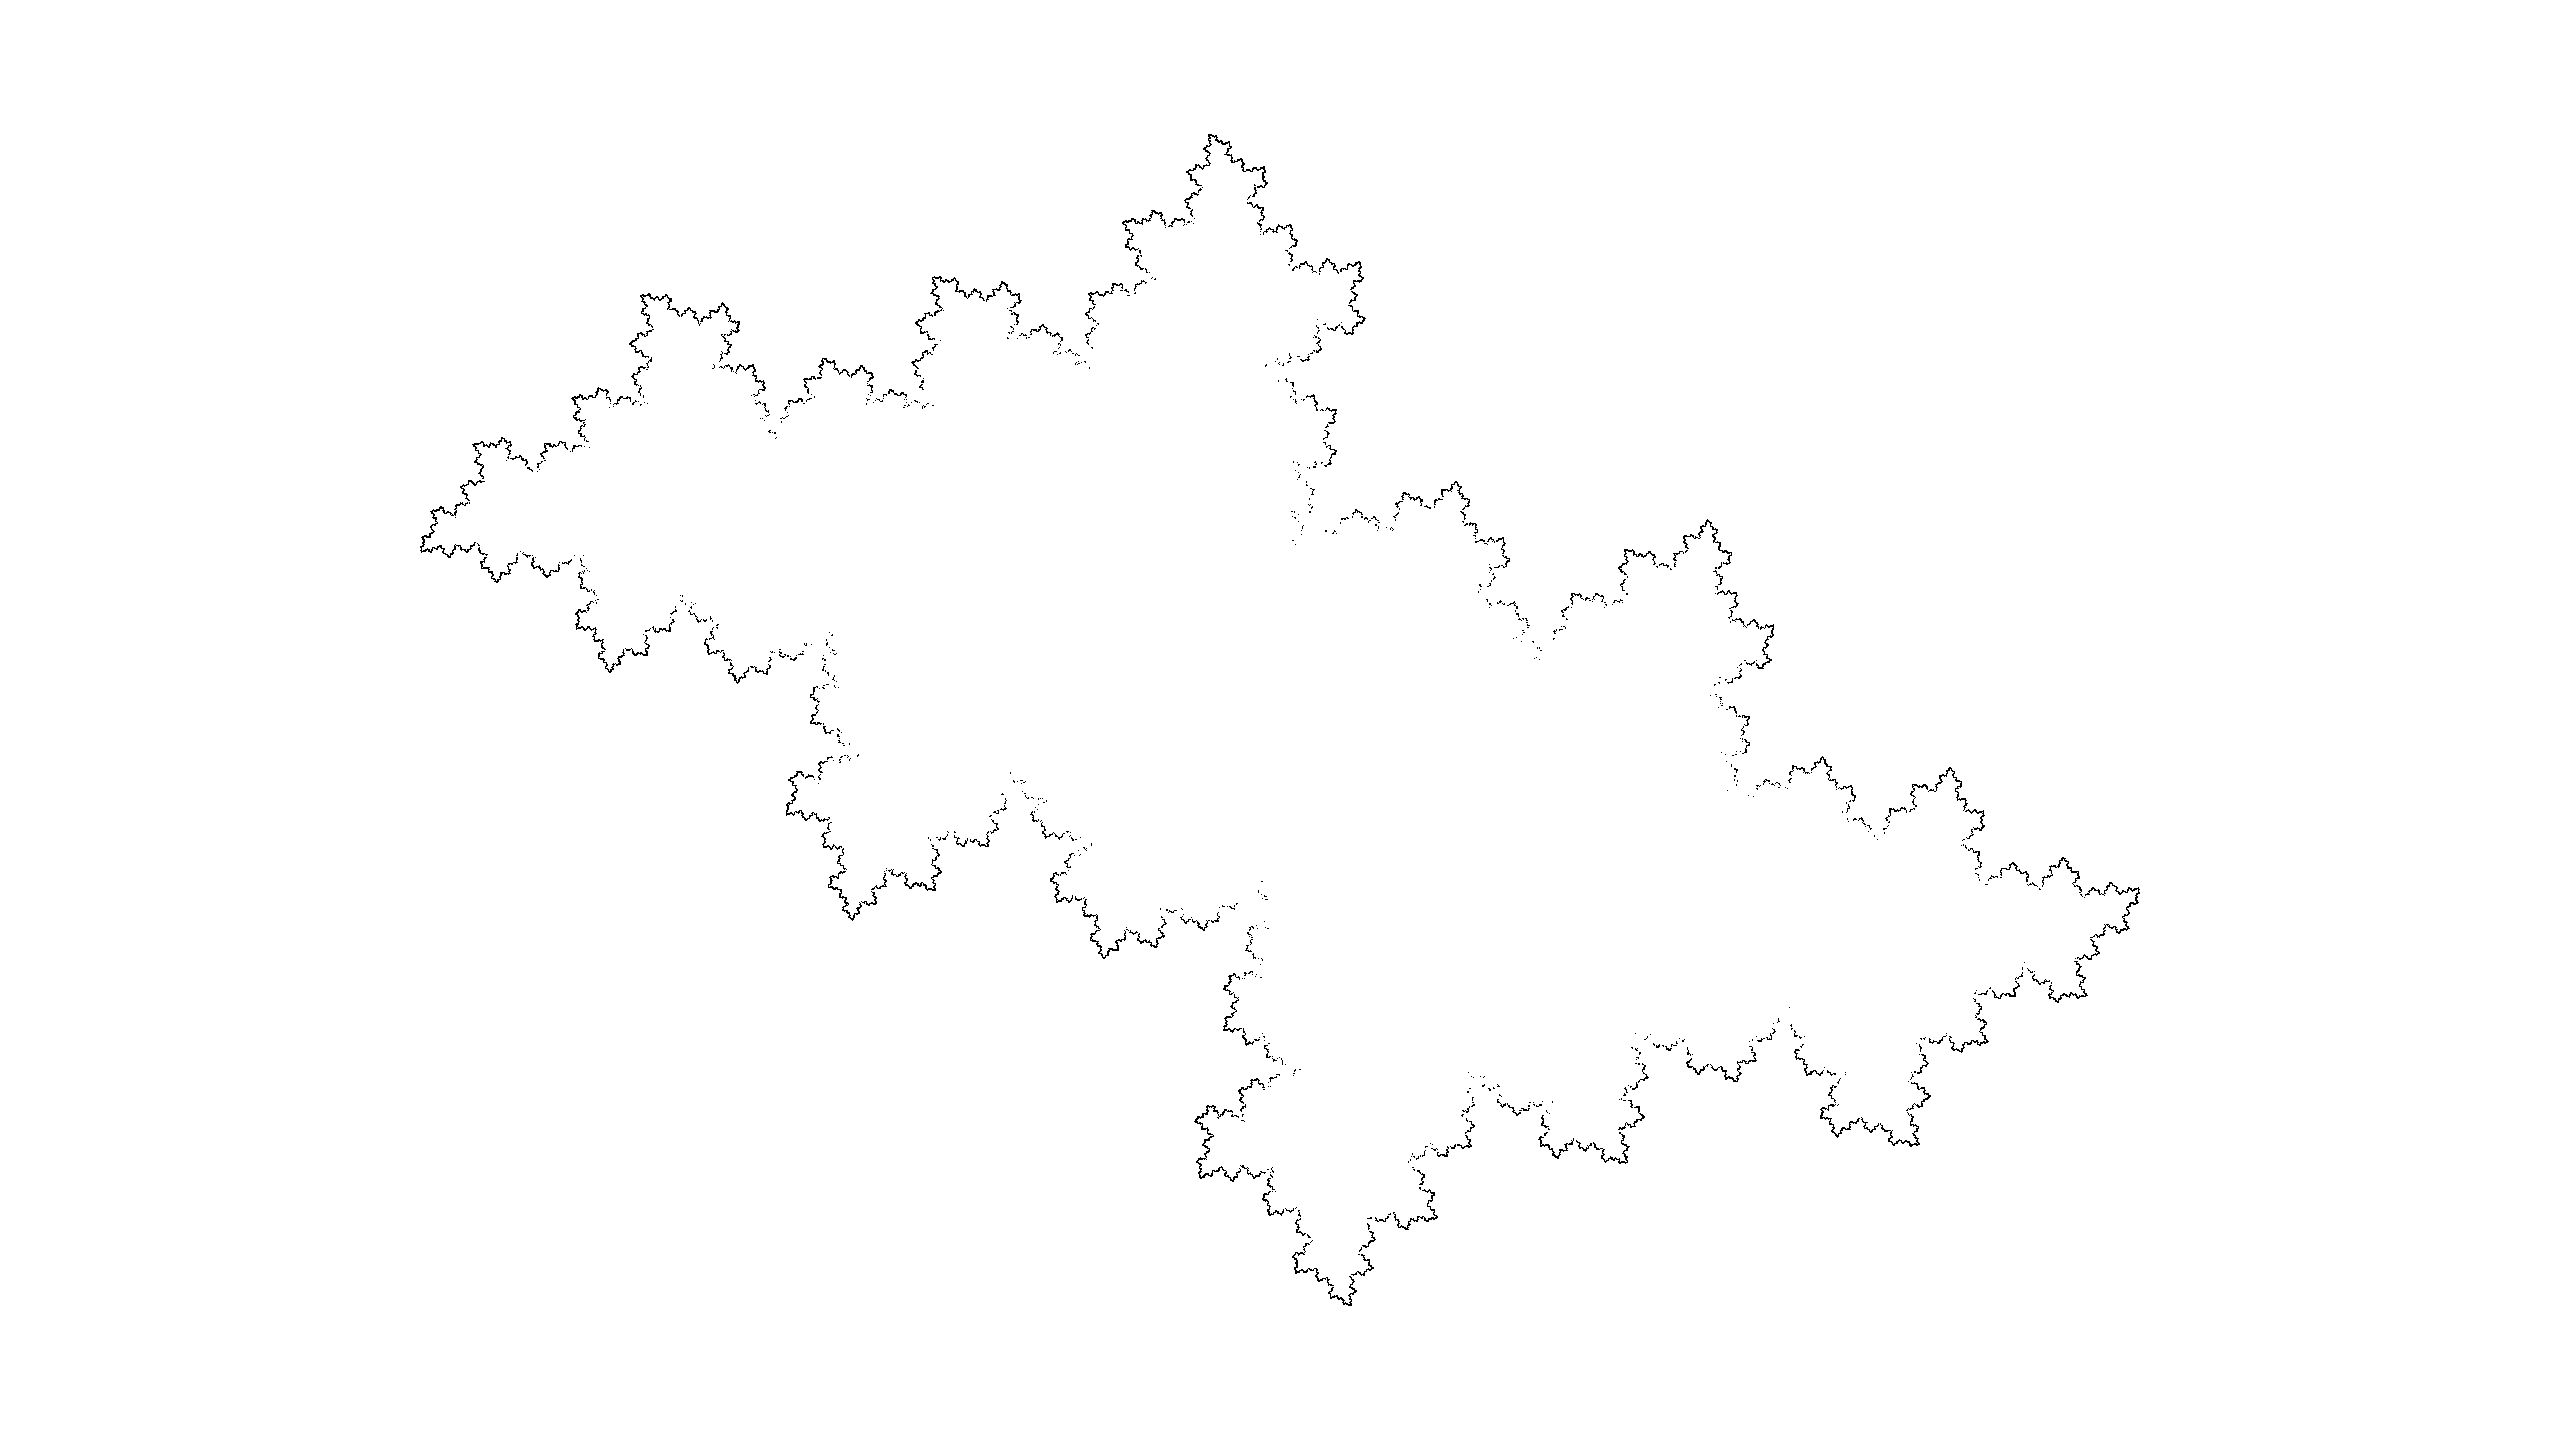
\includegraphics[width=\hsize]{julia/j-b.png}
\end{center}
\caption{Julia-Menge f"ur $c= -0.5+0.5i$}
\end{figure}

\begin{figure}
\begin{center}
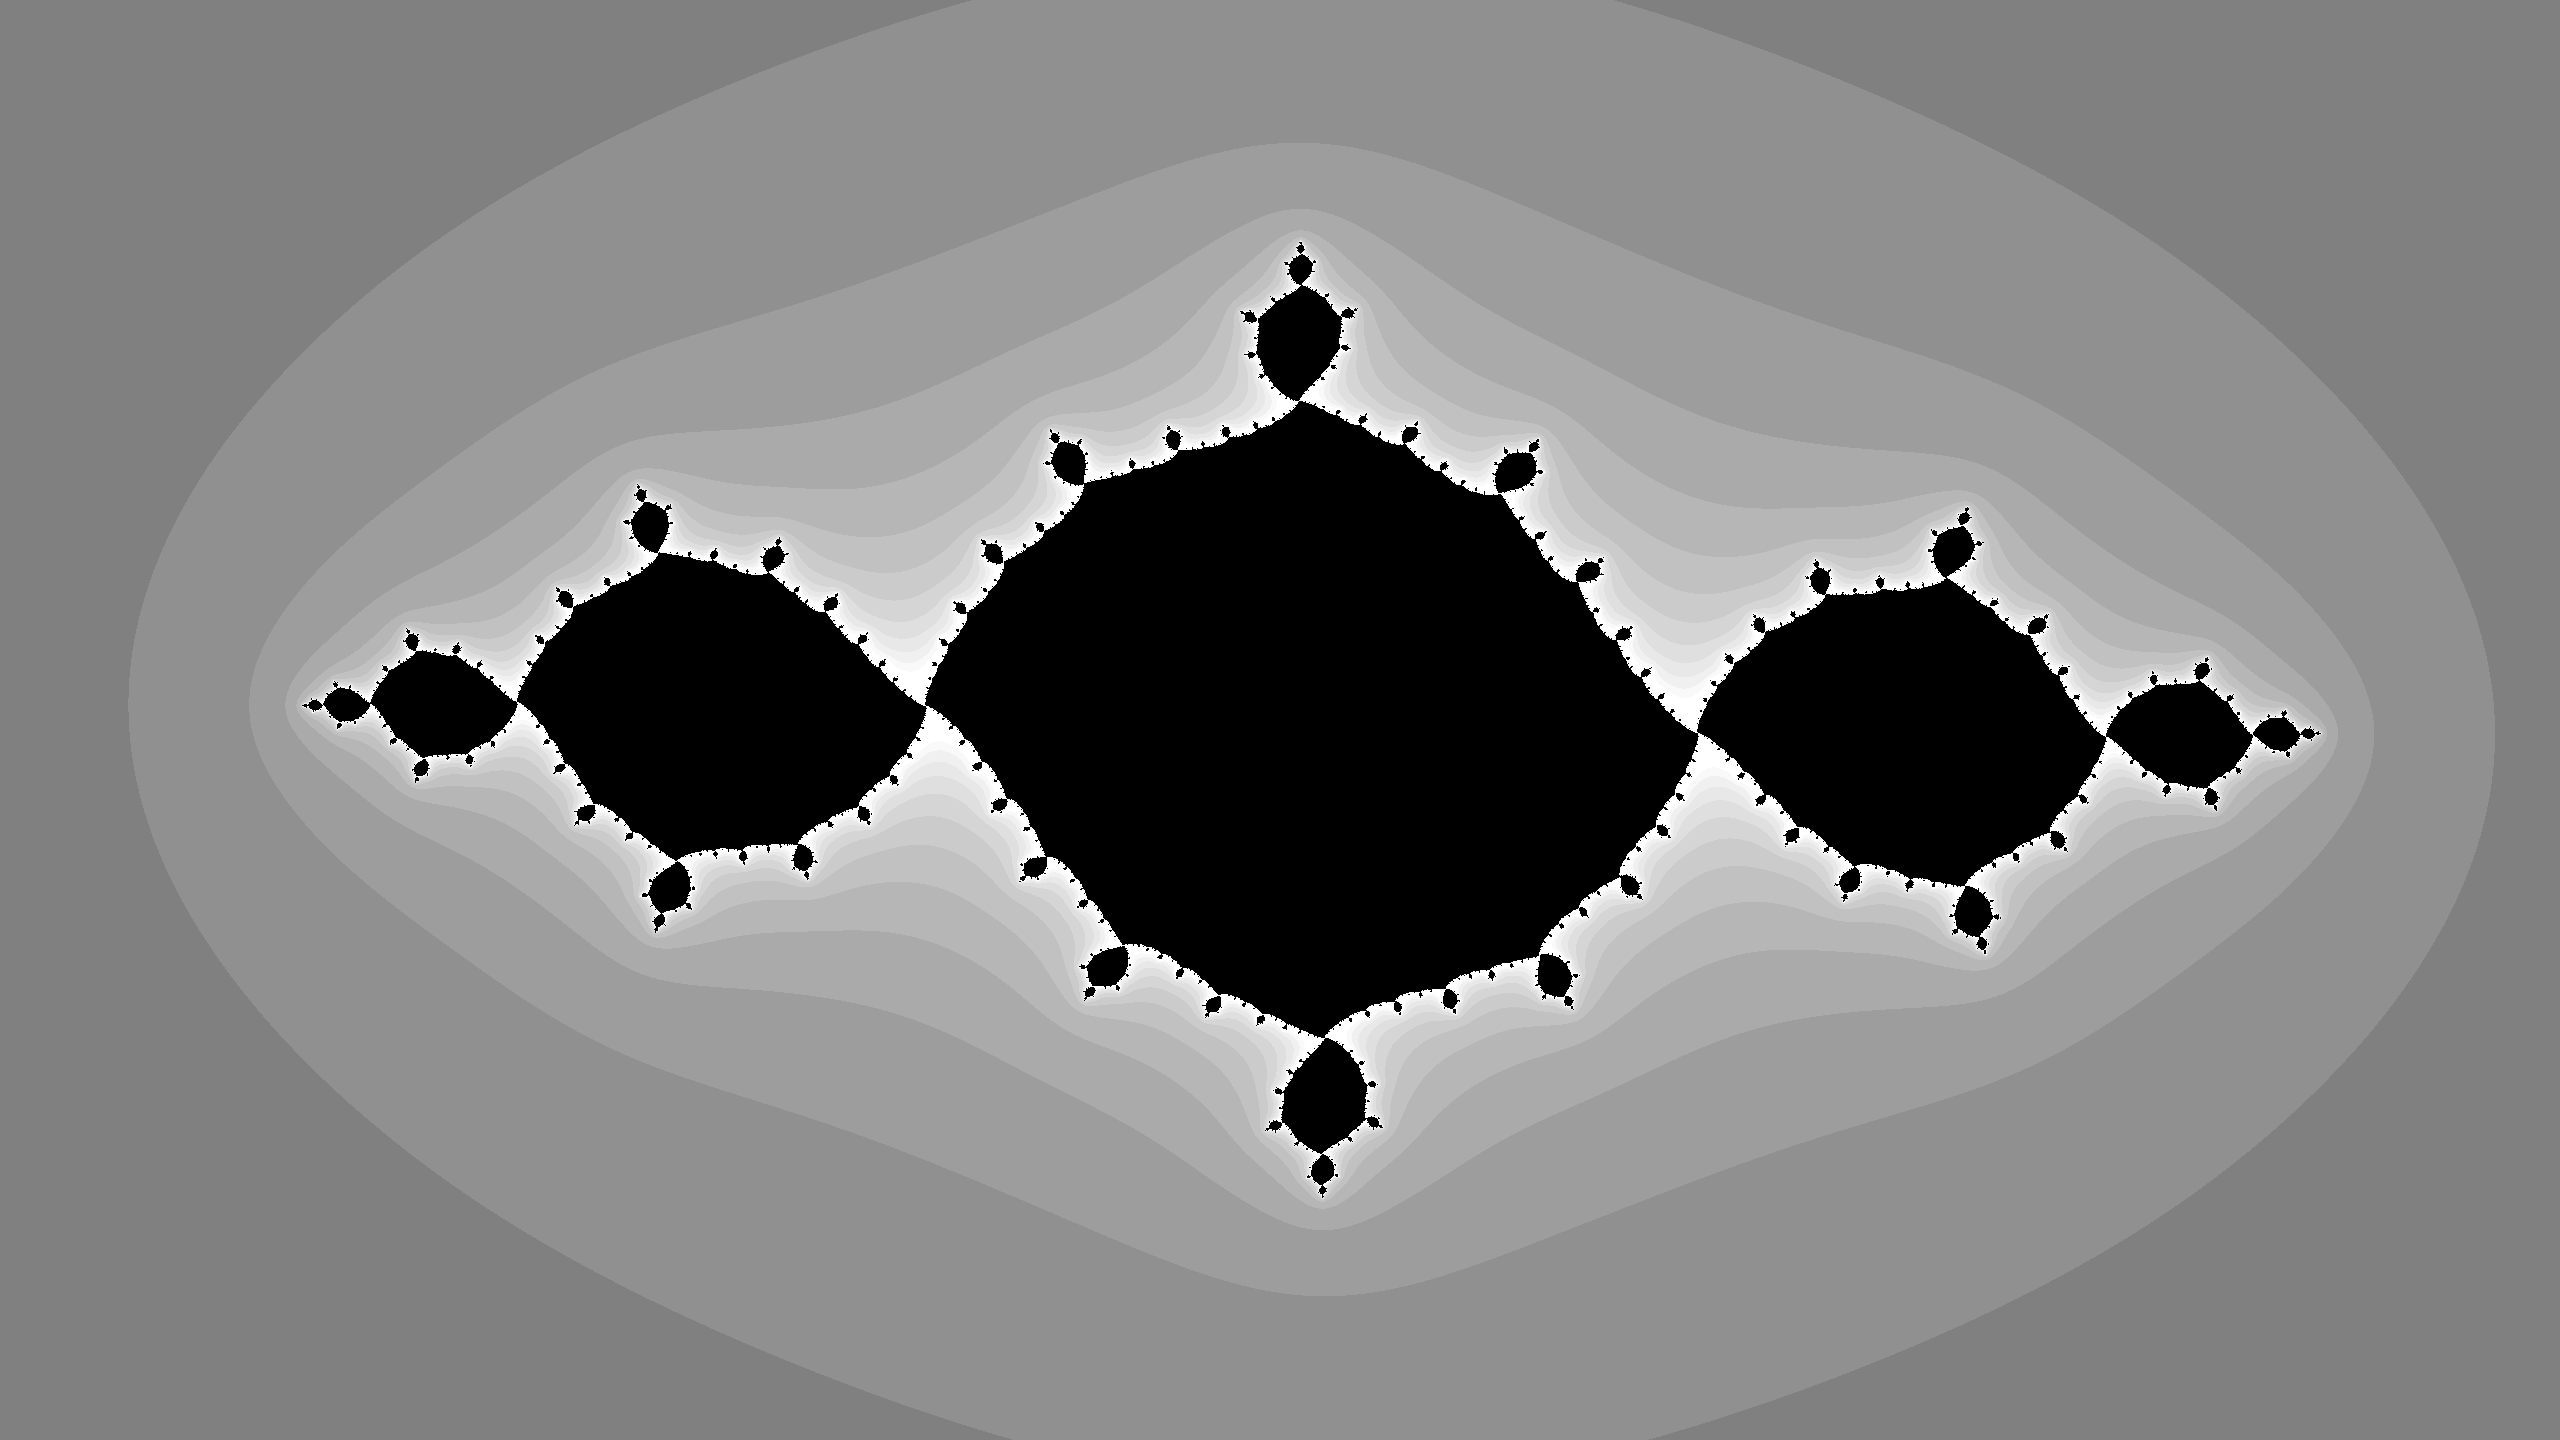
\includegraphics[width=\hsize]{julia/c.png}

\bigskip

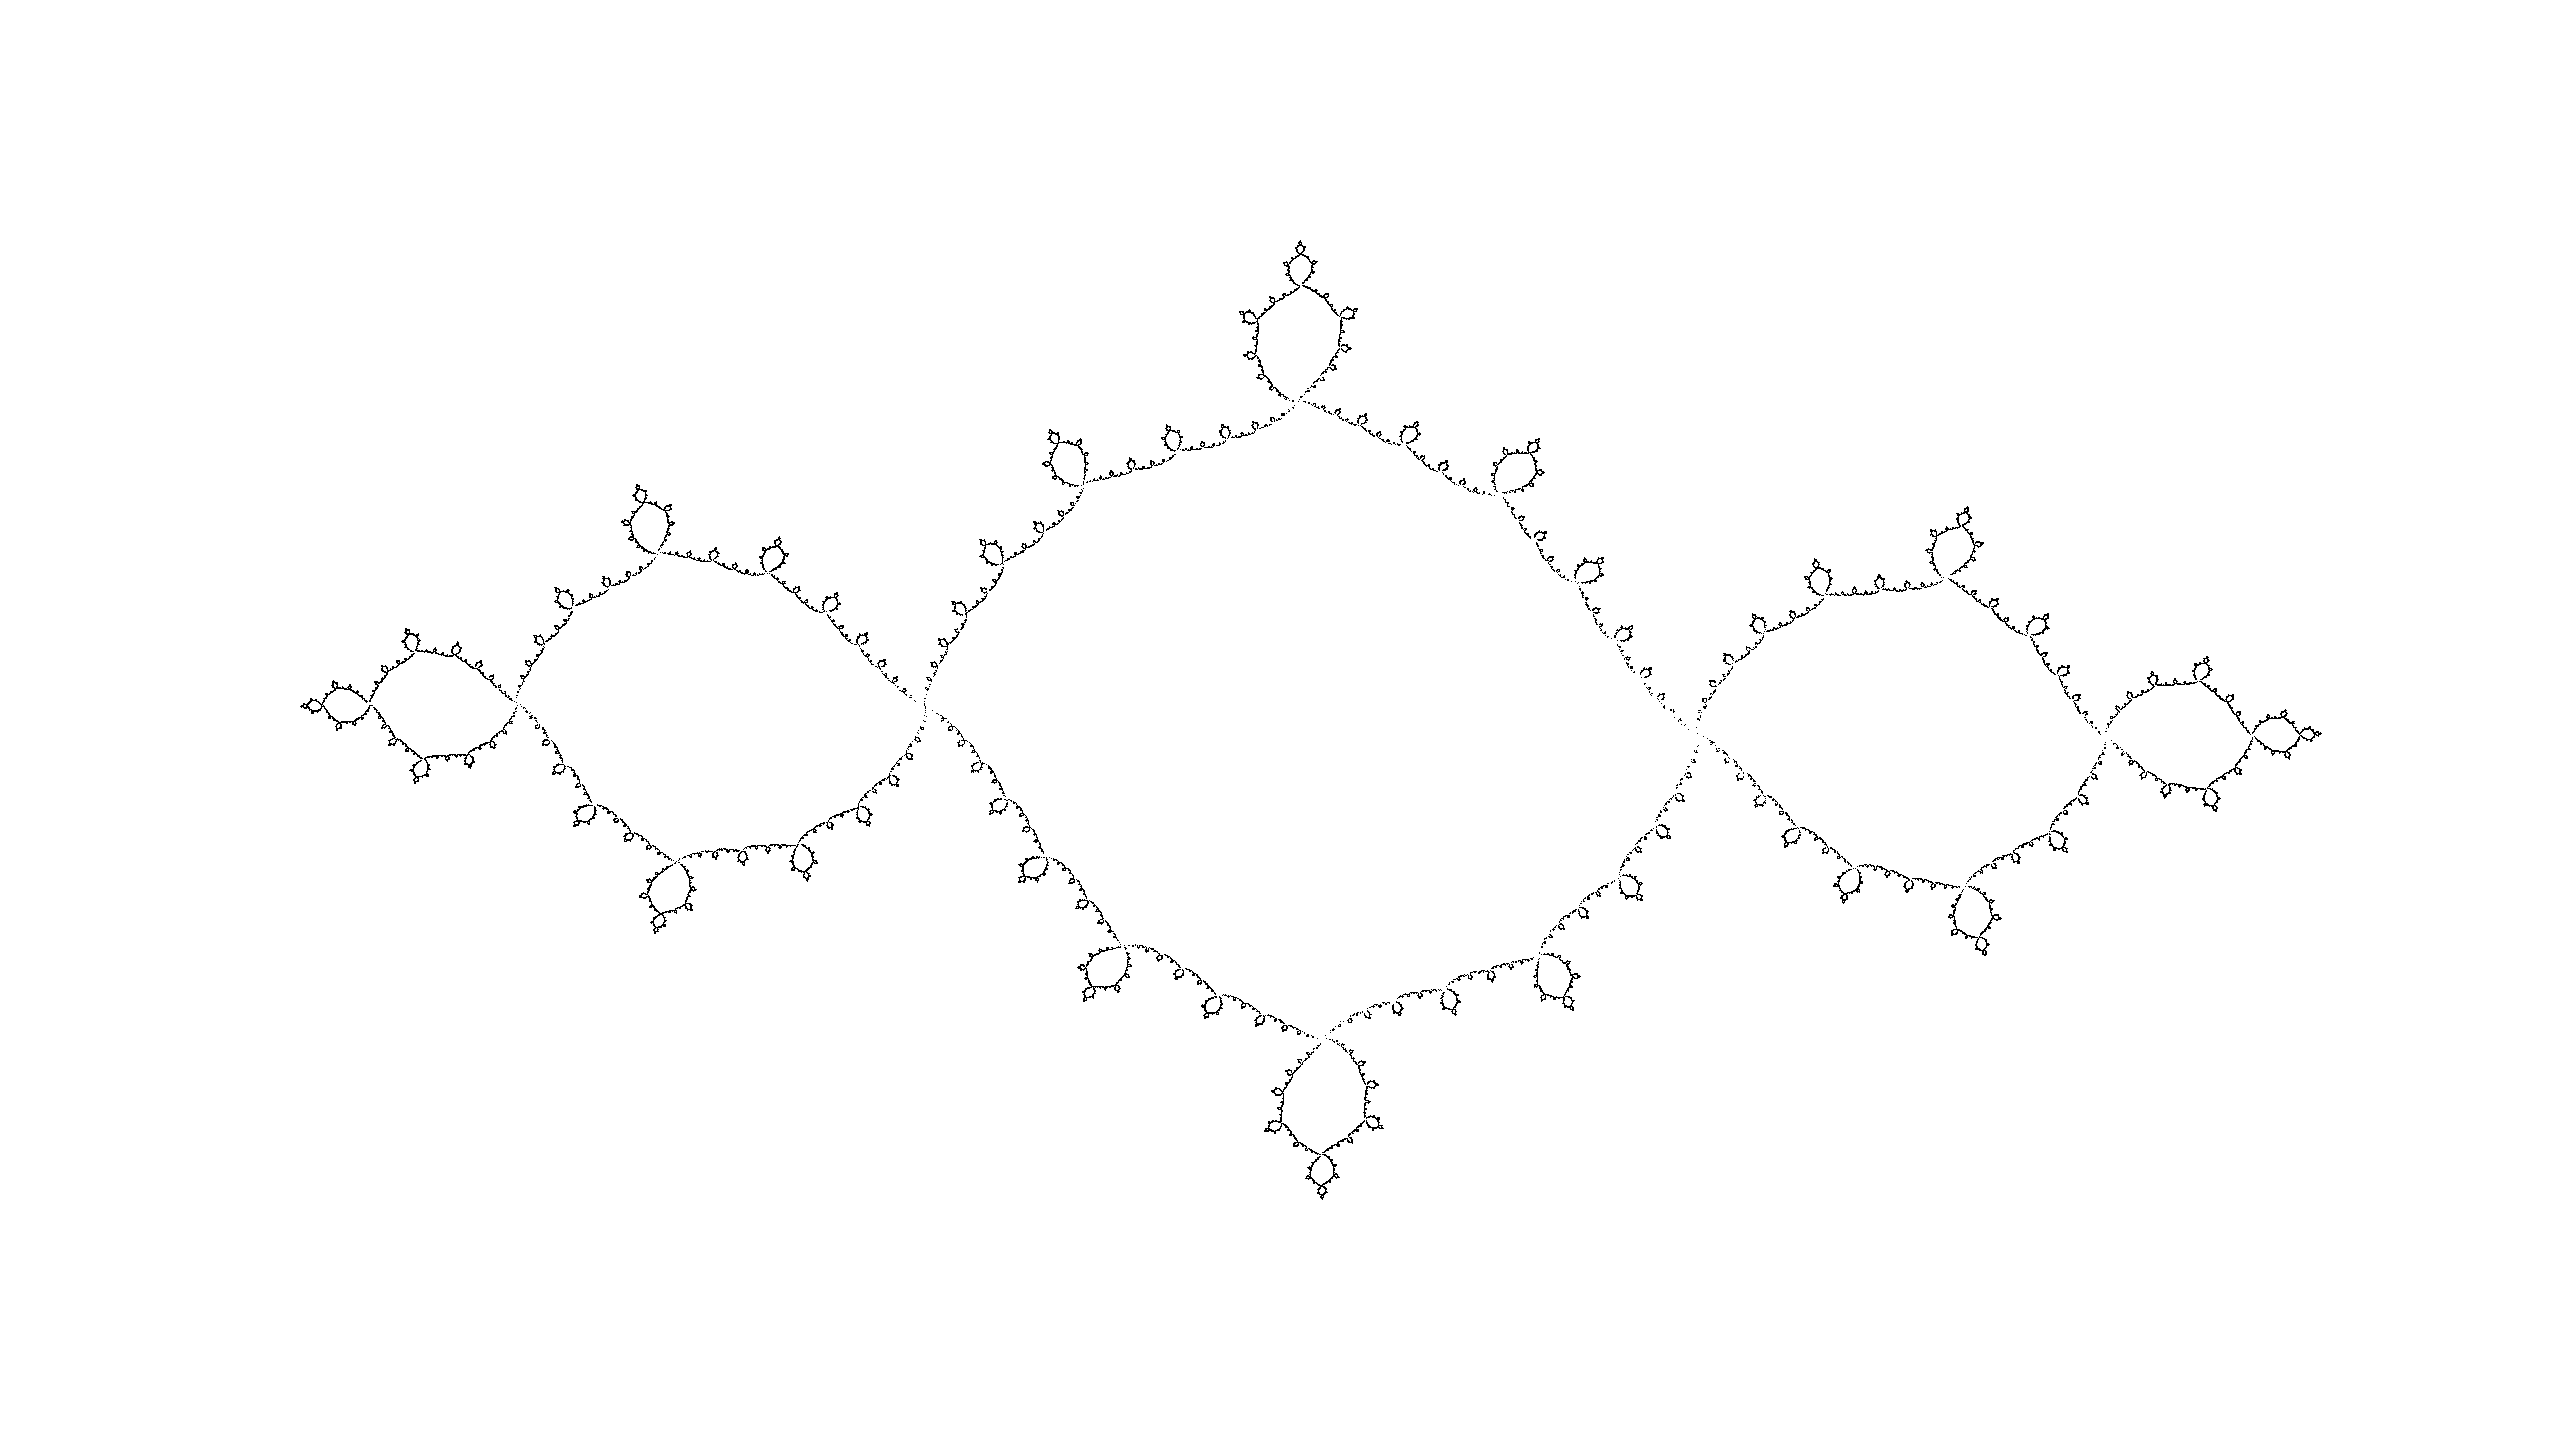
\includegraphics[width=\hsize]{julia/j-c.png}
\end{center}
\caption{Julia-Menge f"ur $c= -1+0.05i$}
\end{figure}

\begin{figure}
\begin{center}
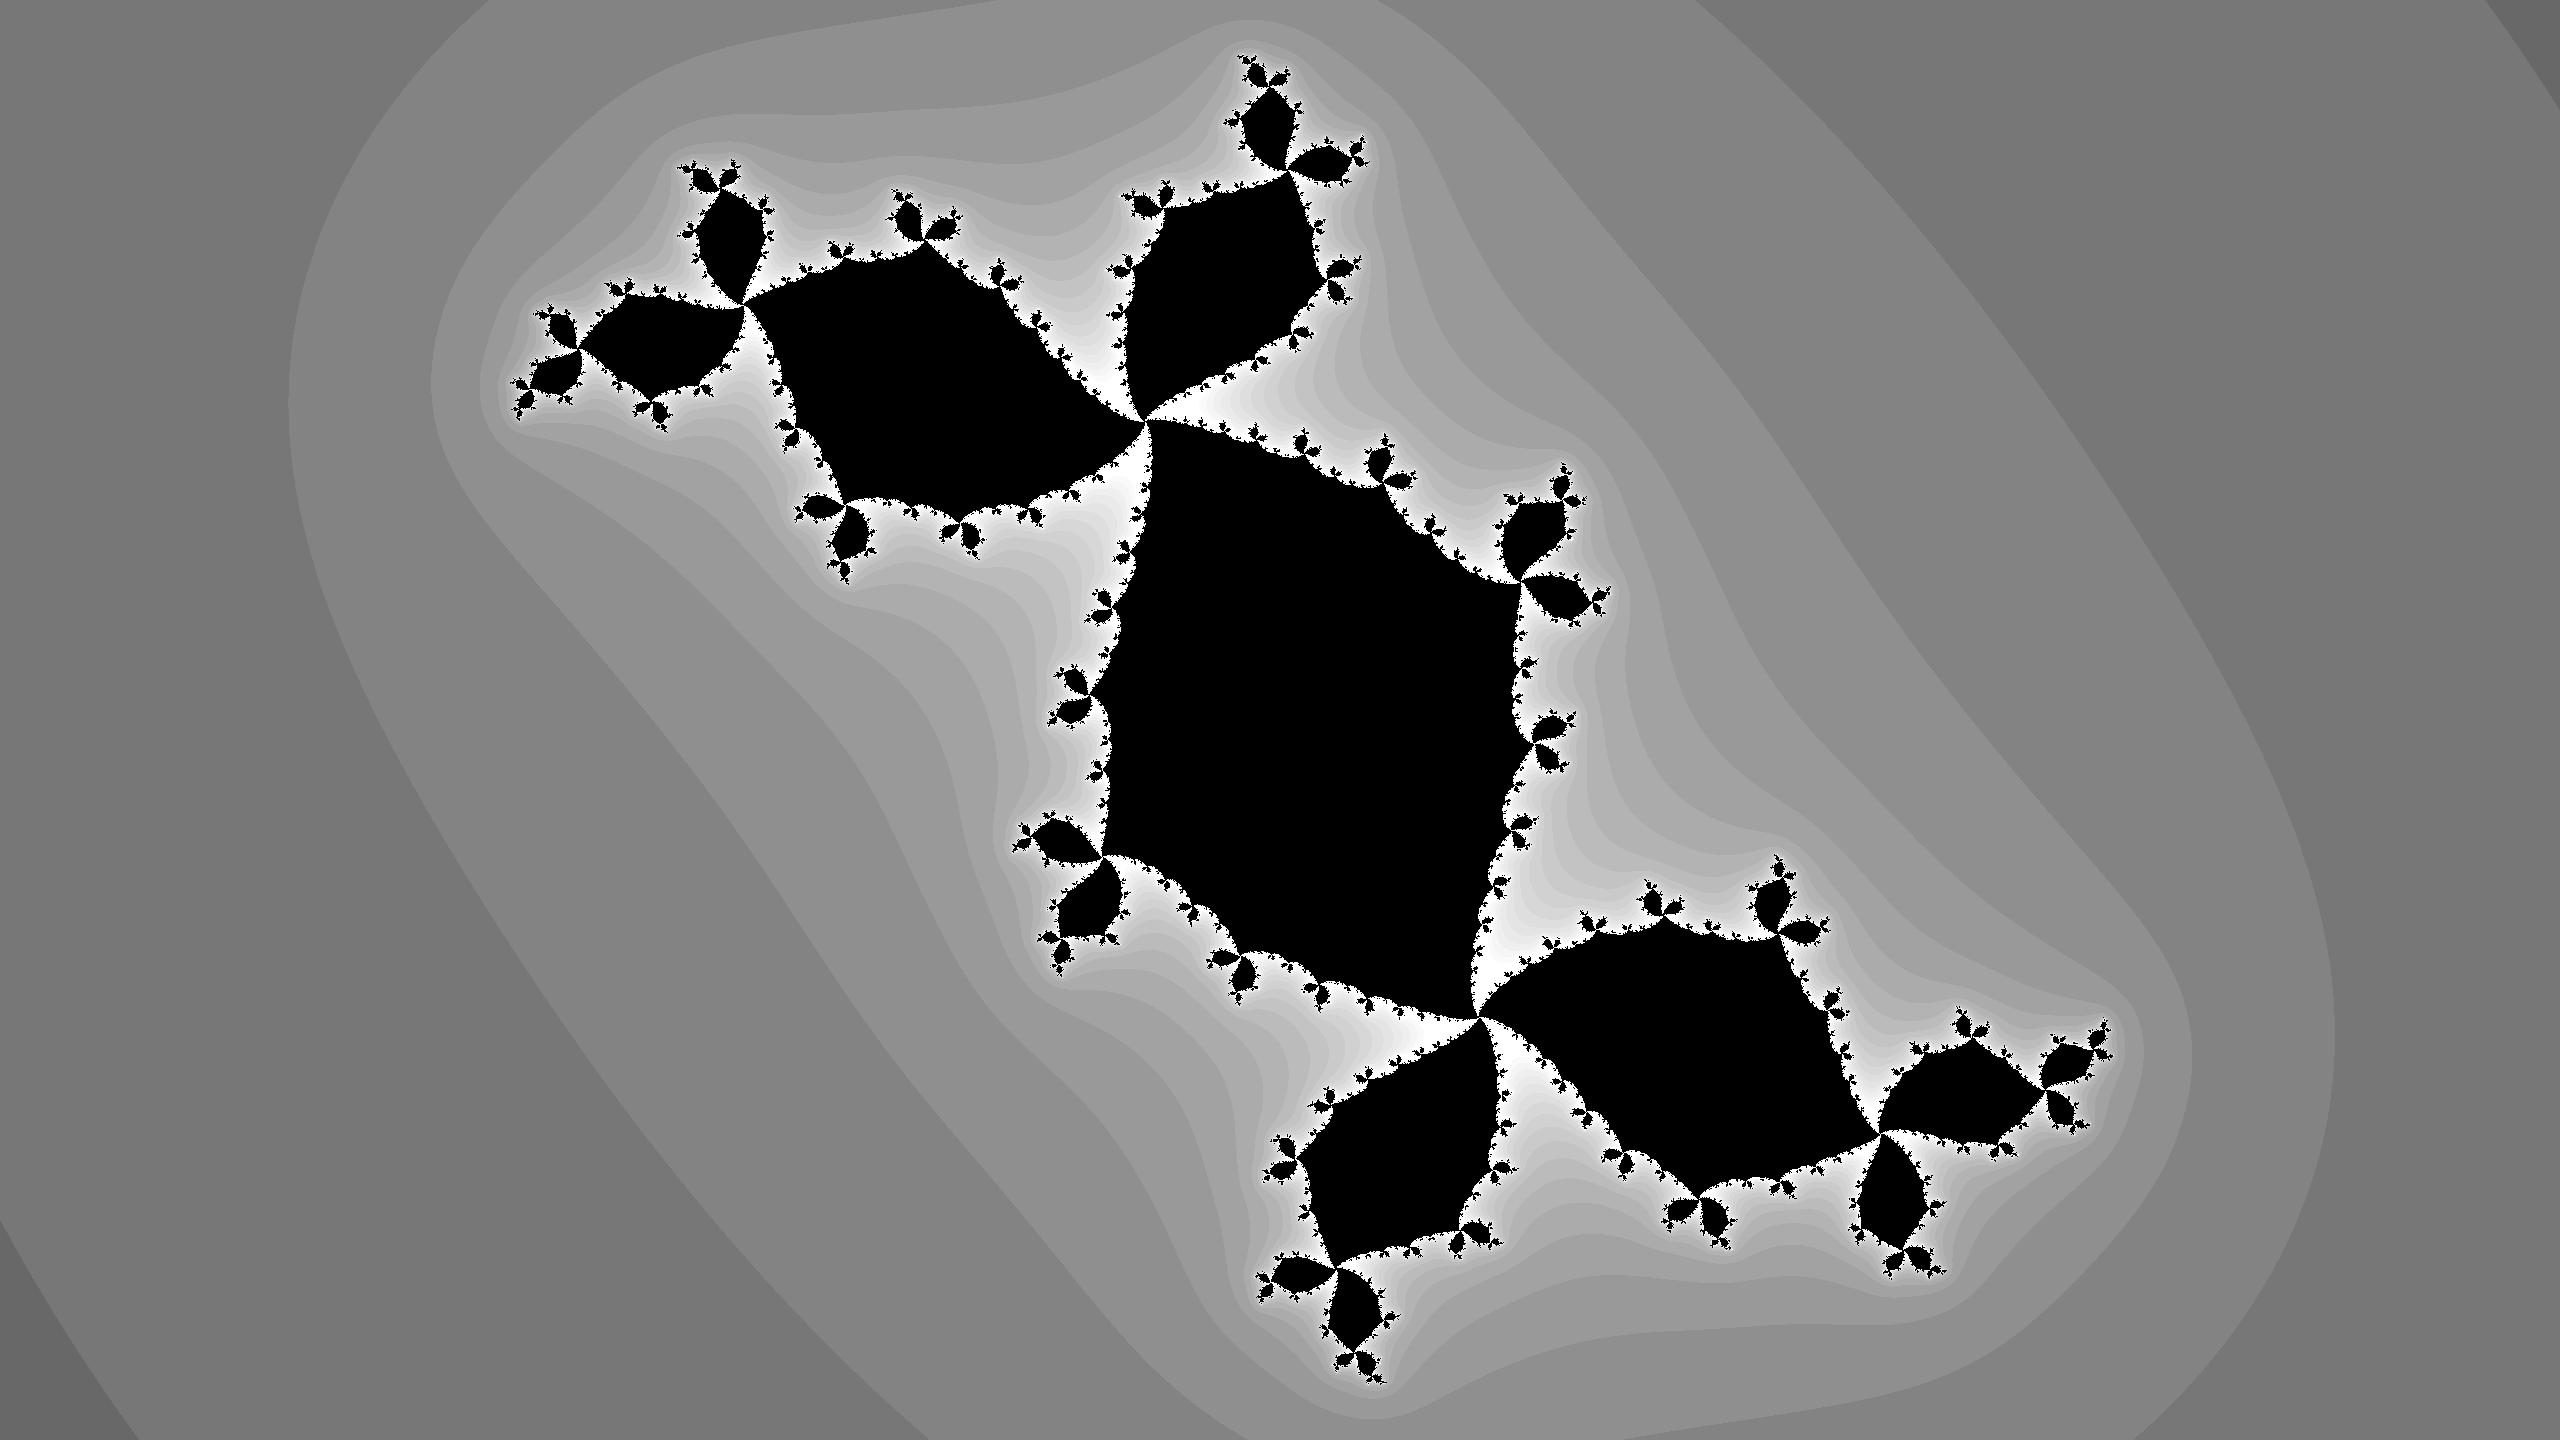
\includegraphics[width=\hsize]{julia/d.png}

\bigskip

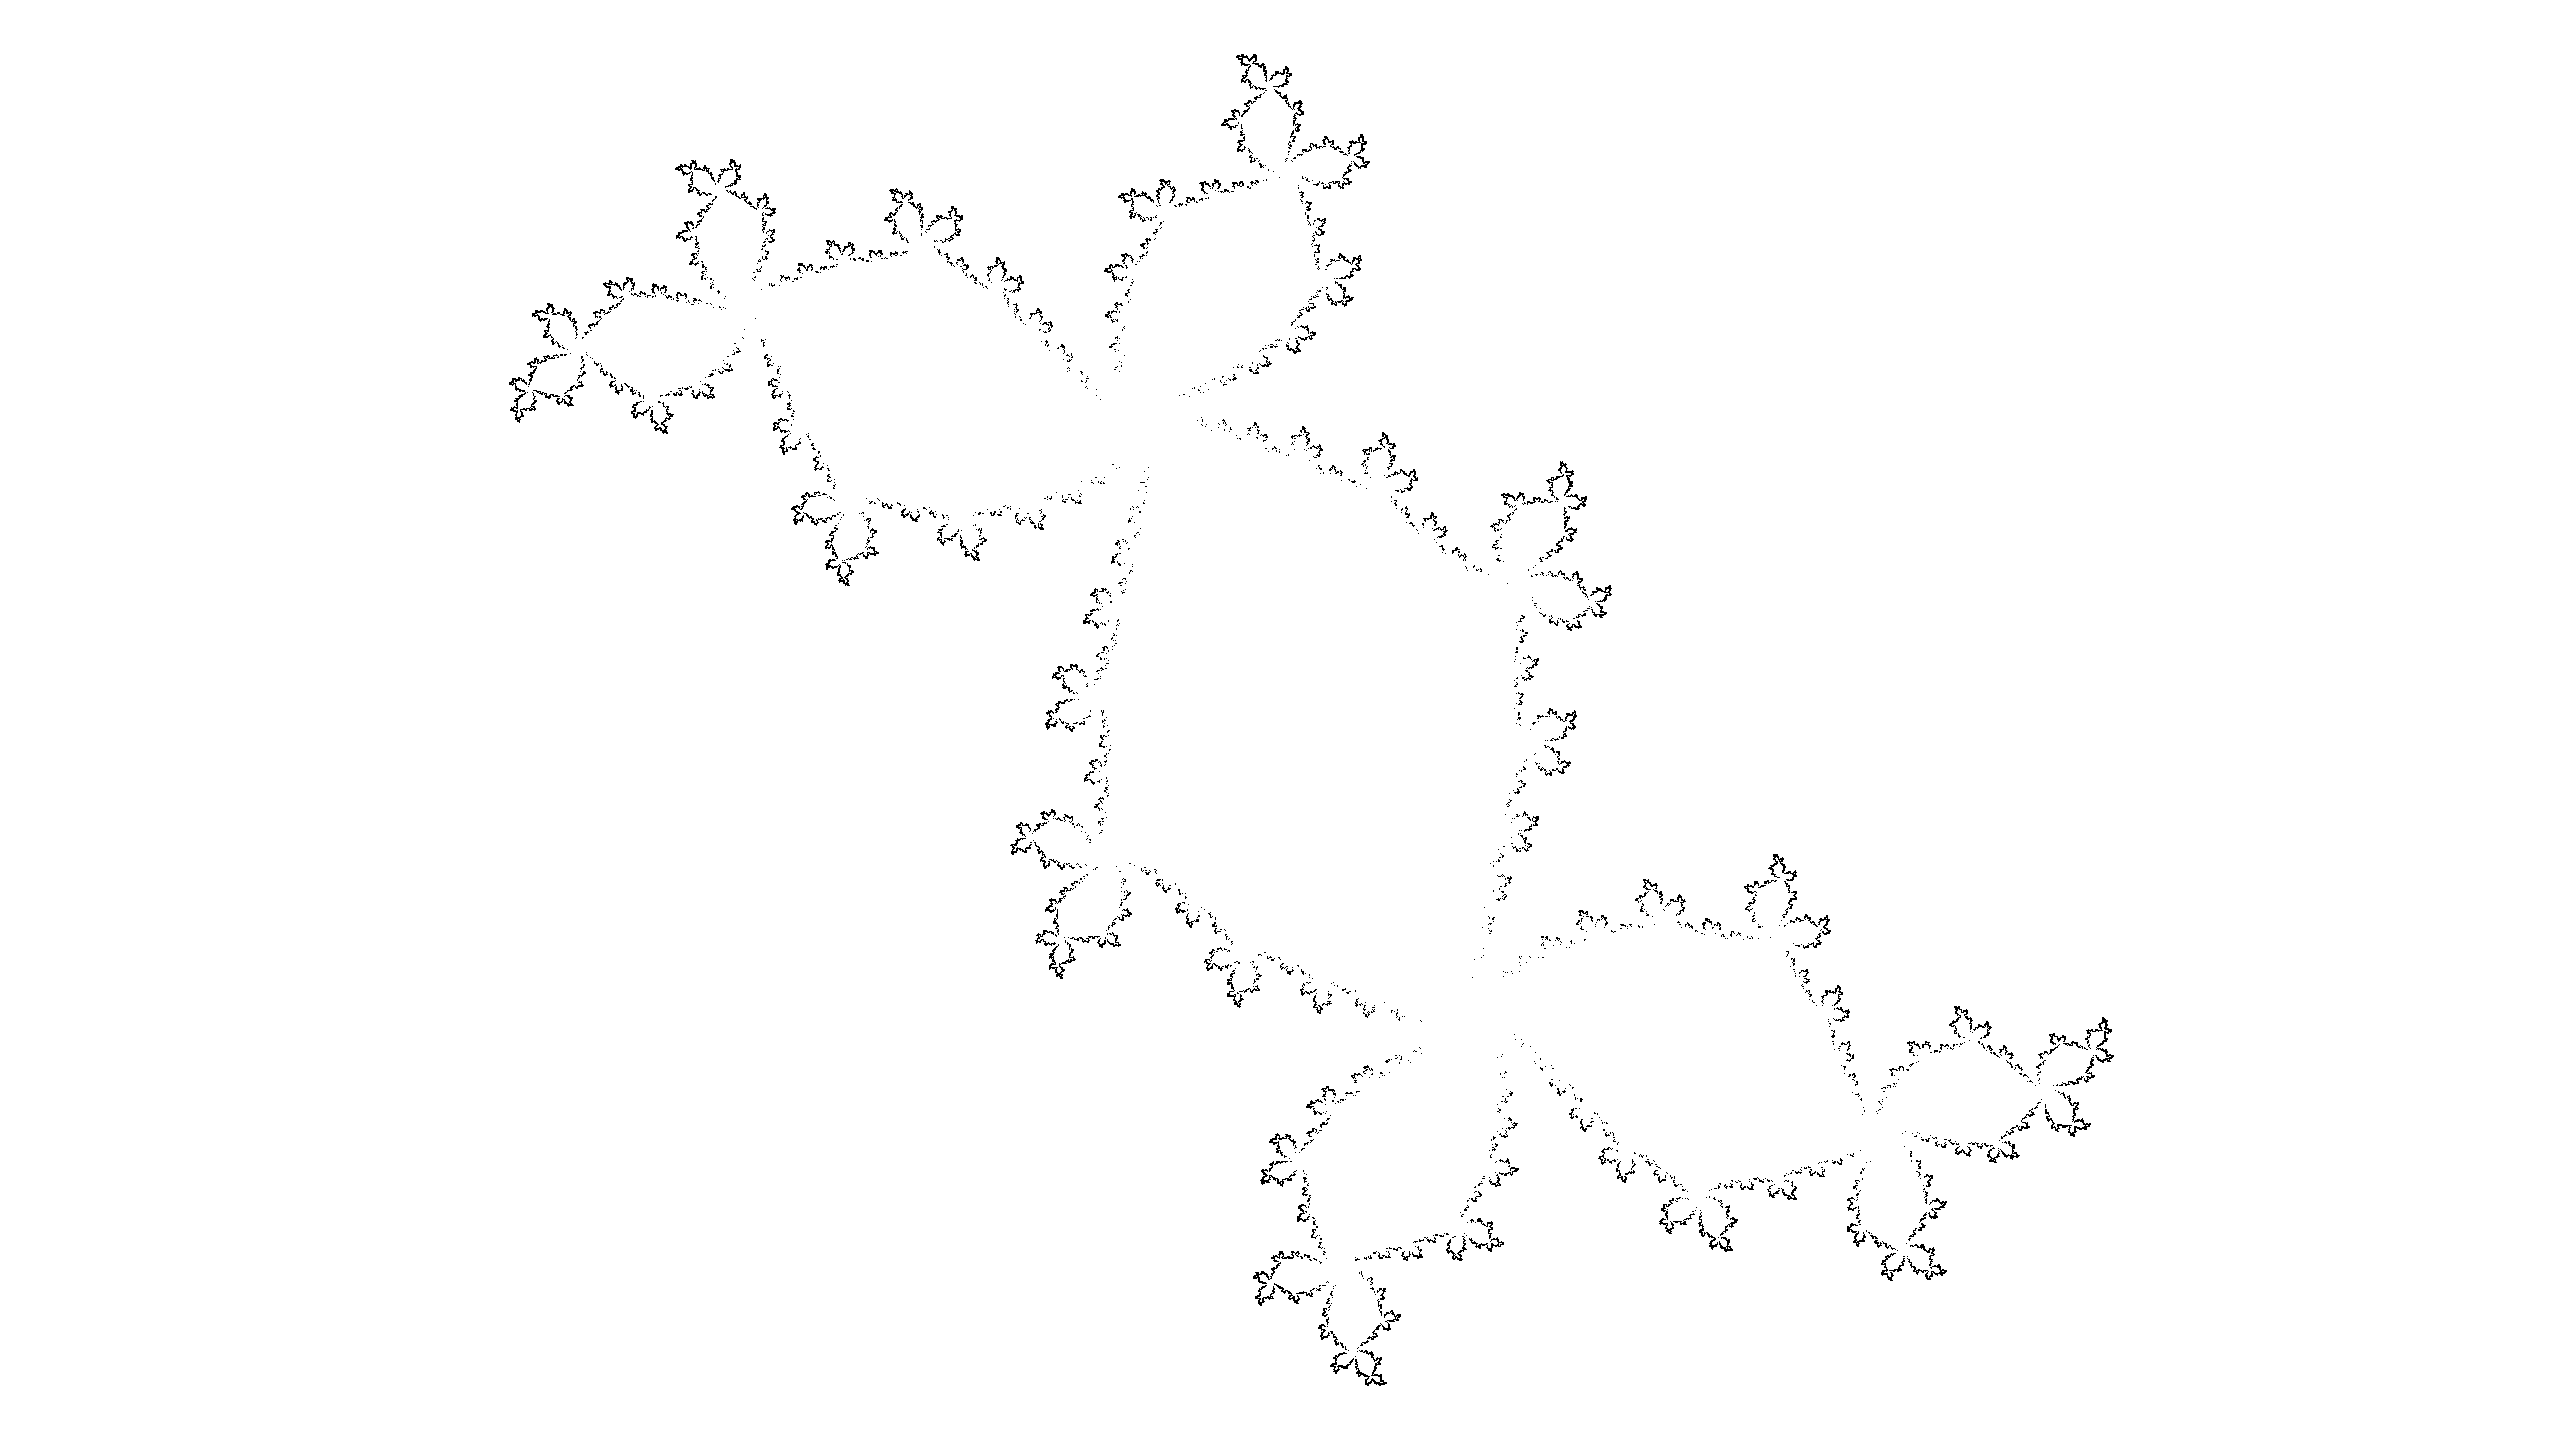
\includegraphics[width=\hsize]{julia/j-d.png}
\end{center}
\caption{Julia-Menge f"ur $c= -0.1+0.75i$}
\end{figure}

\begin{figure}
\begin{center}
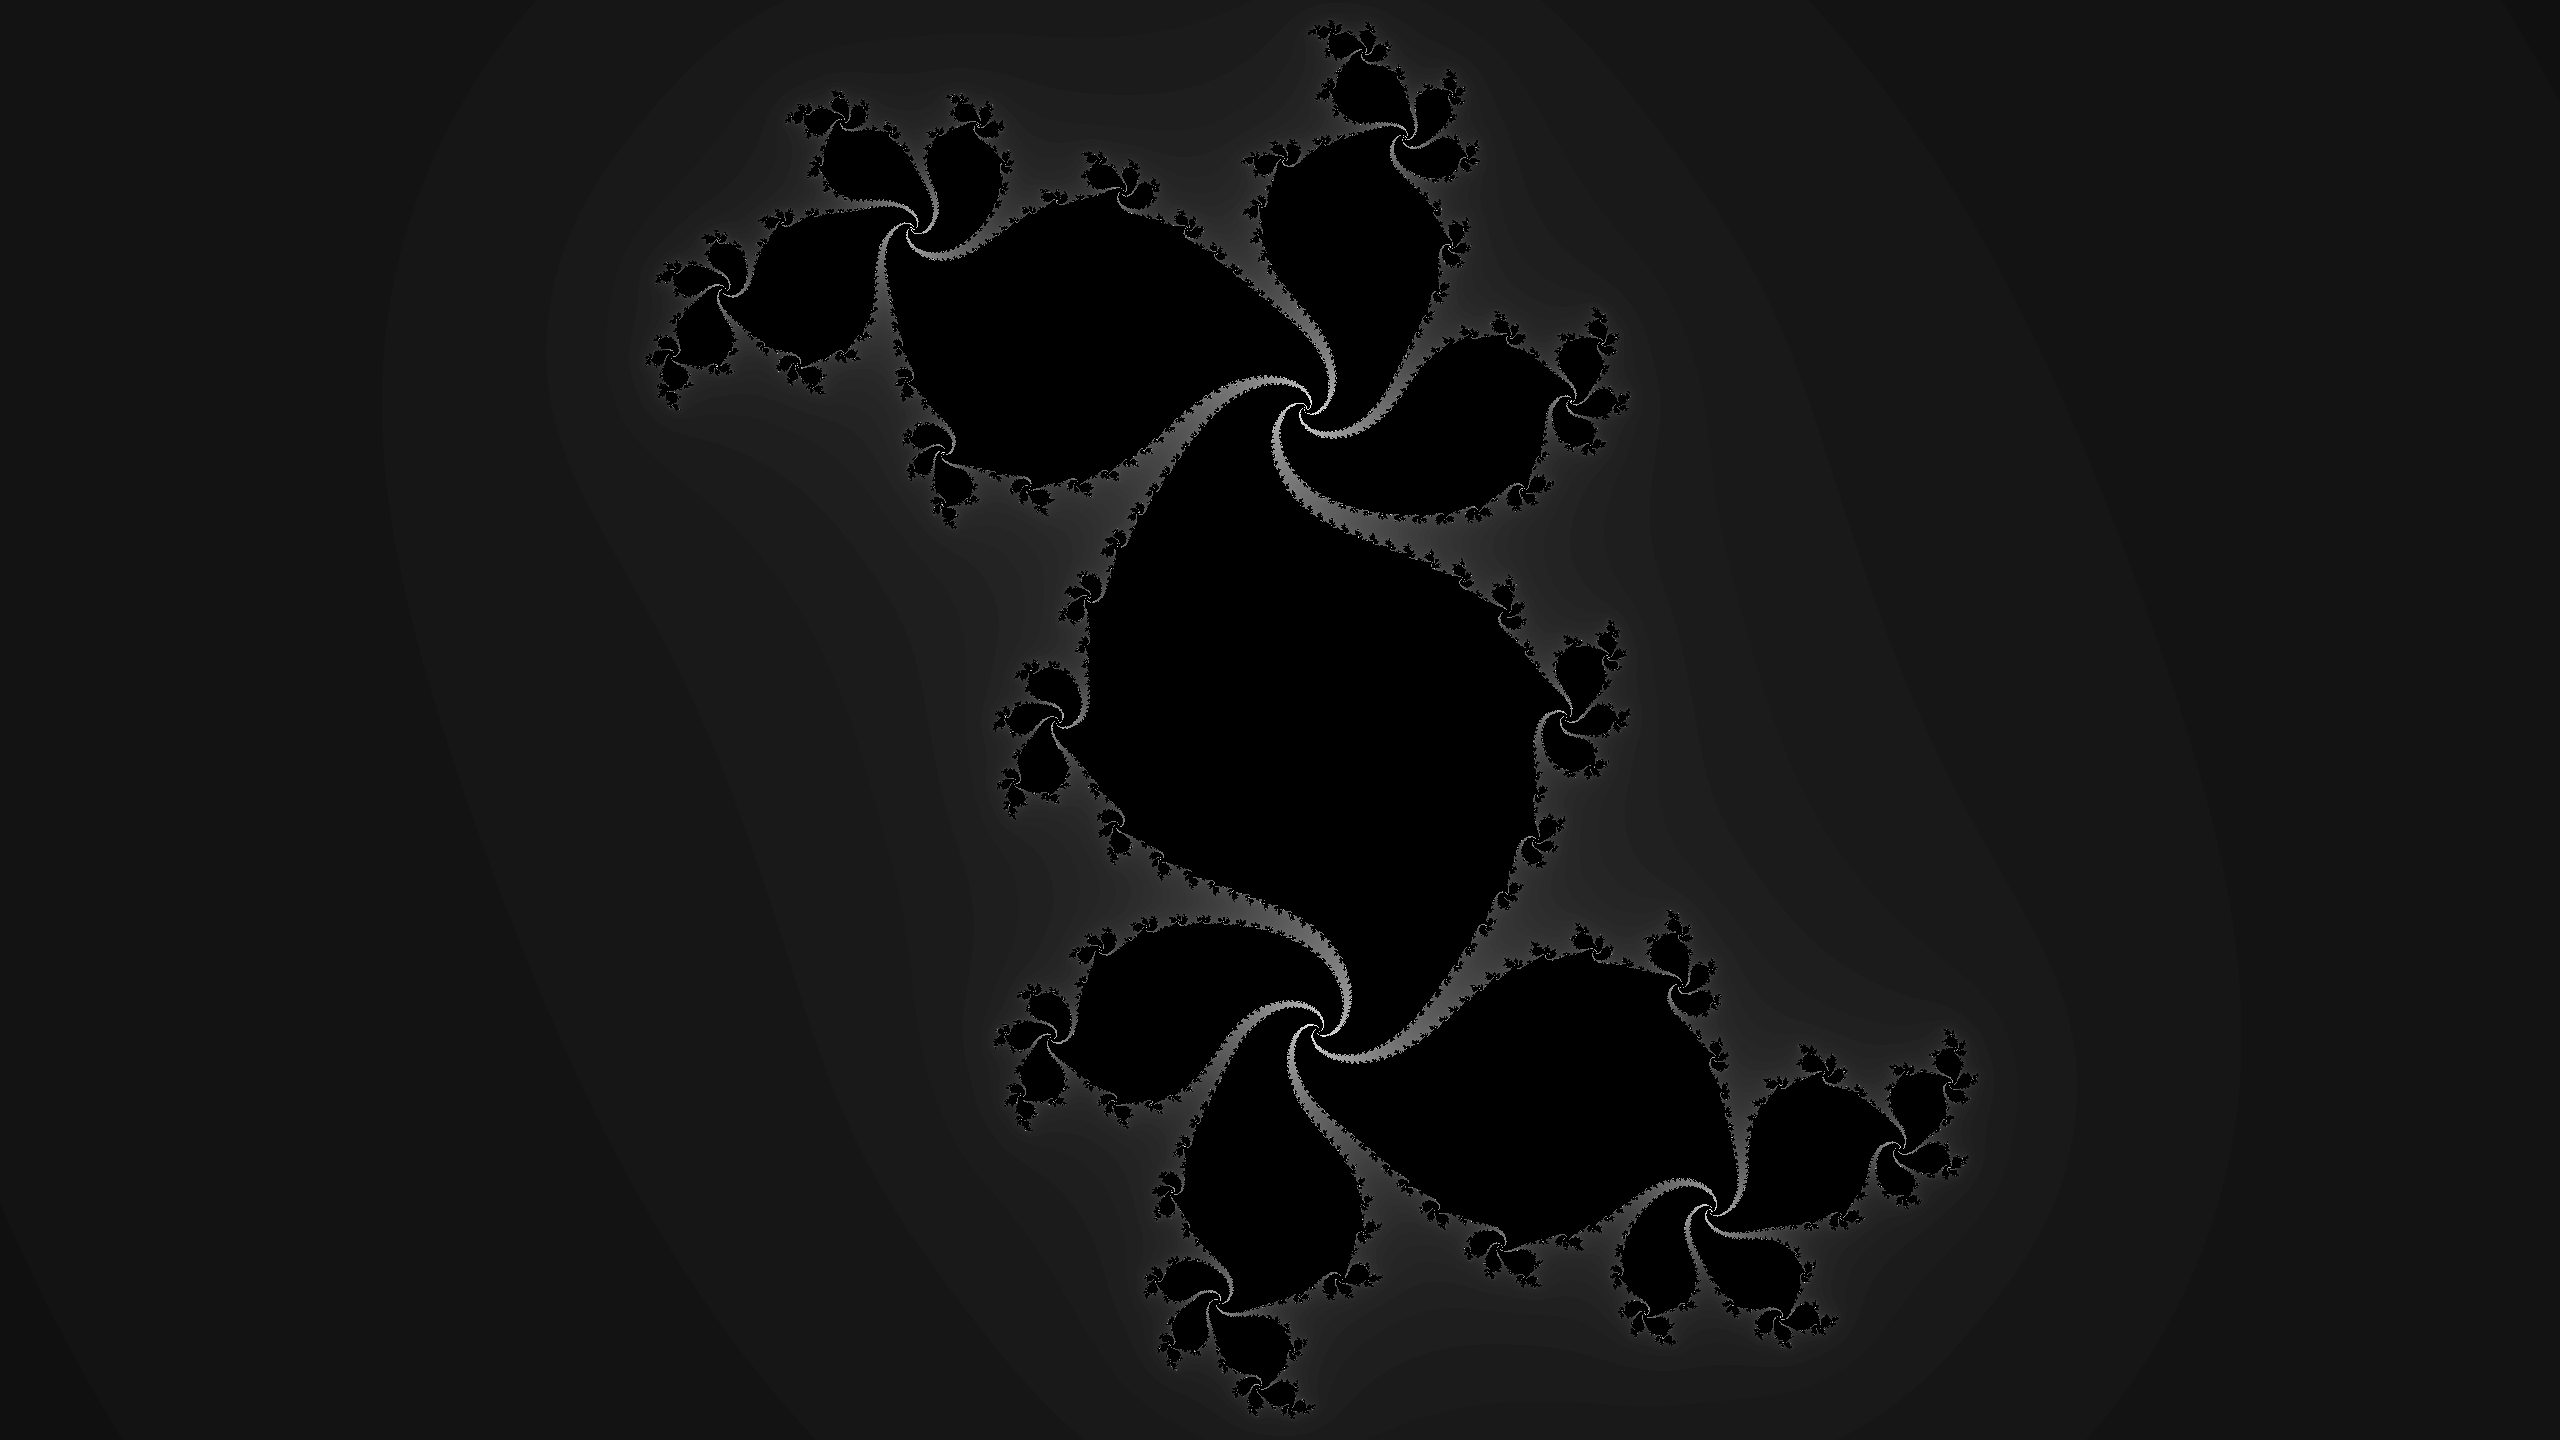
\includegraphics[width=\hsize]{julia/e.png}

\bigskip

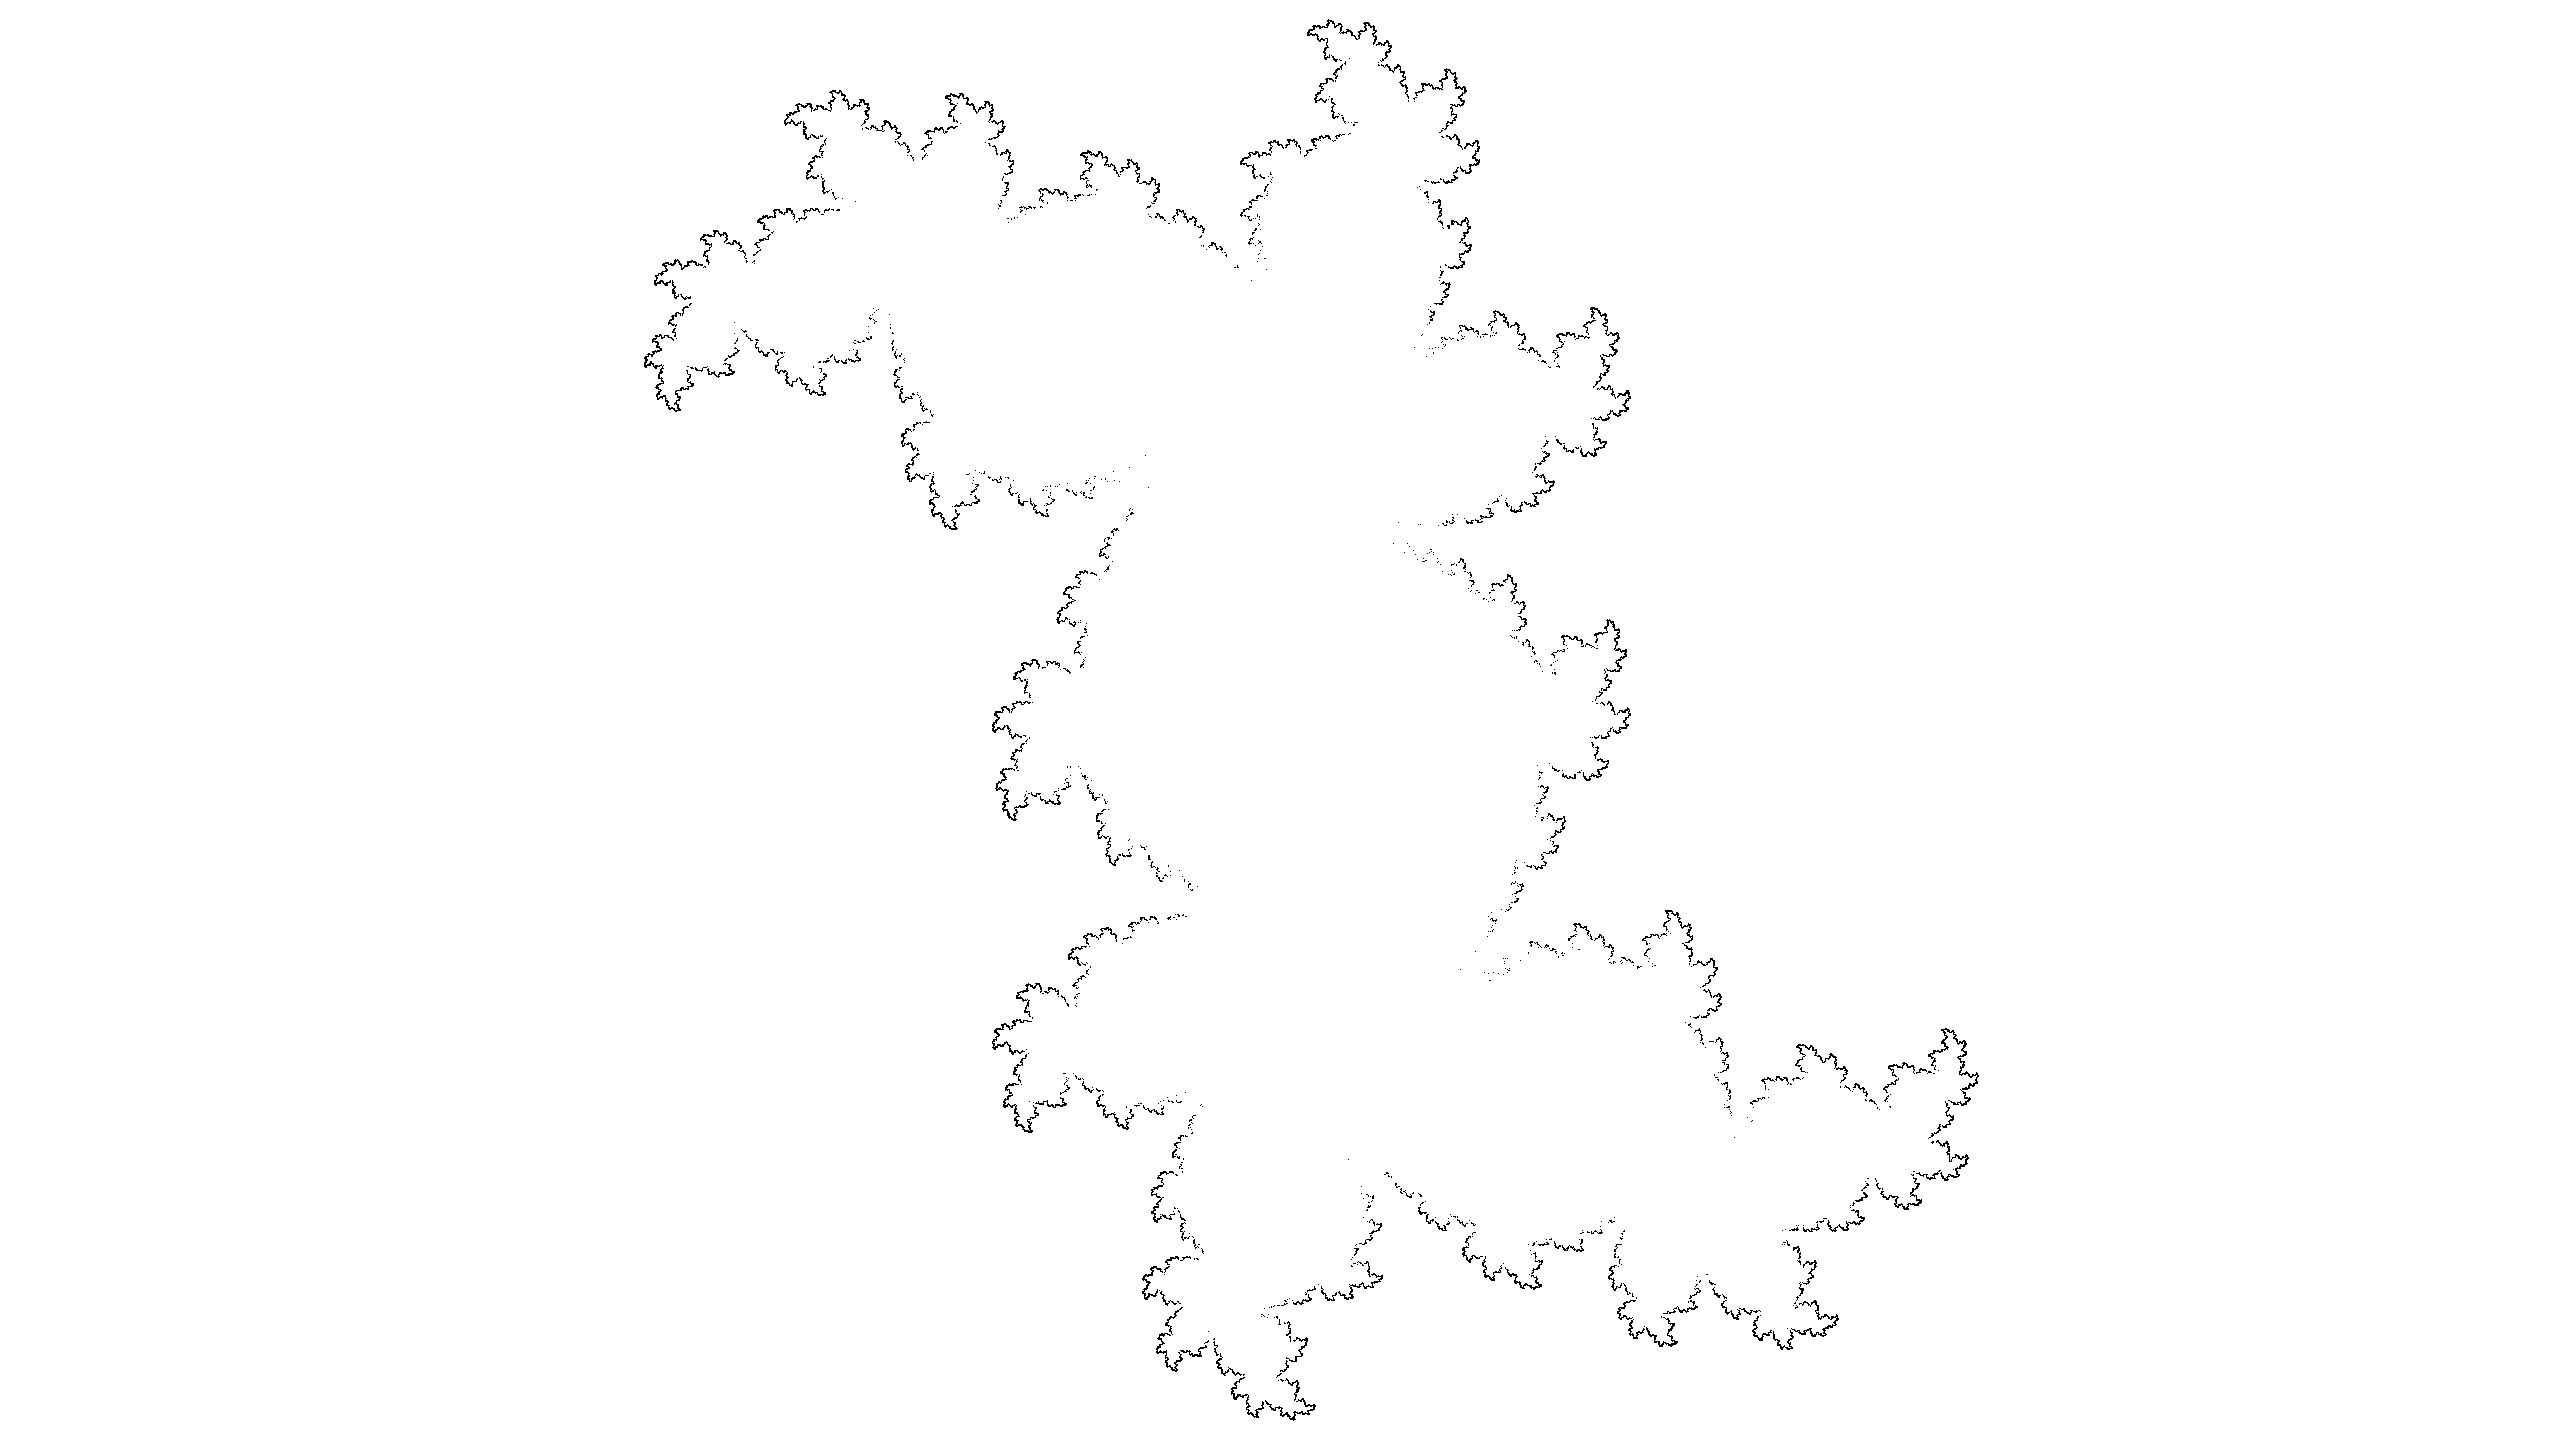
\includegraphics[width=\hsize]{julia/j-e.png}
\end{center}
\caption{Julia-Menge f"ur $c= 0.25+0.52i$}
\end{figure}

\begin{figure}
\begin{center}
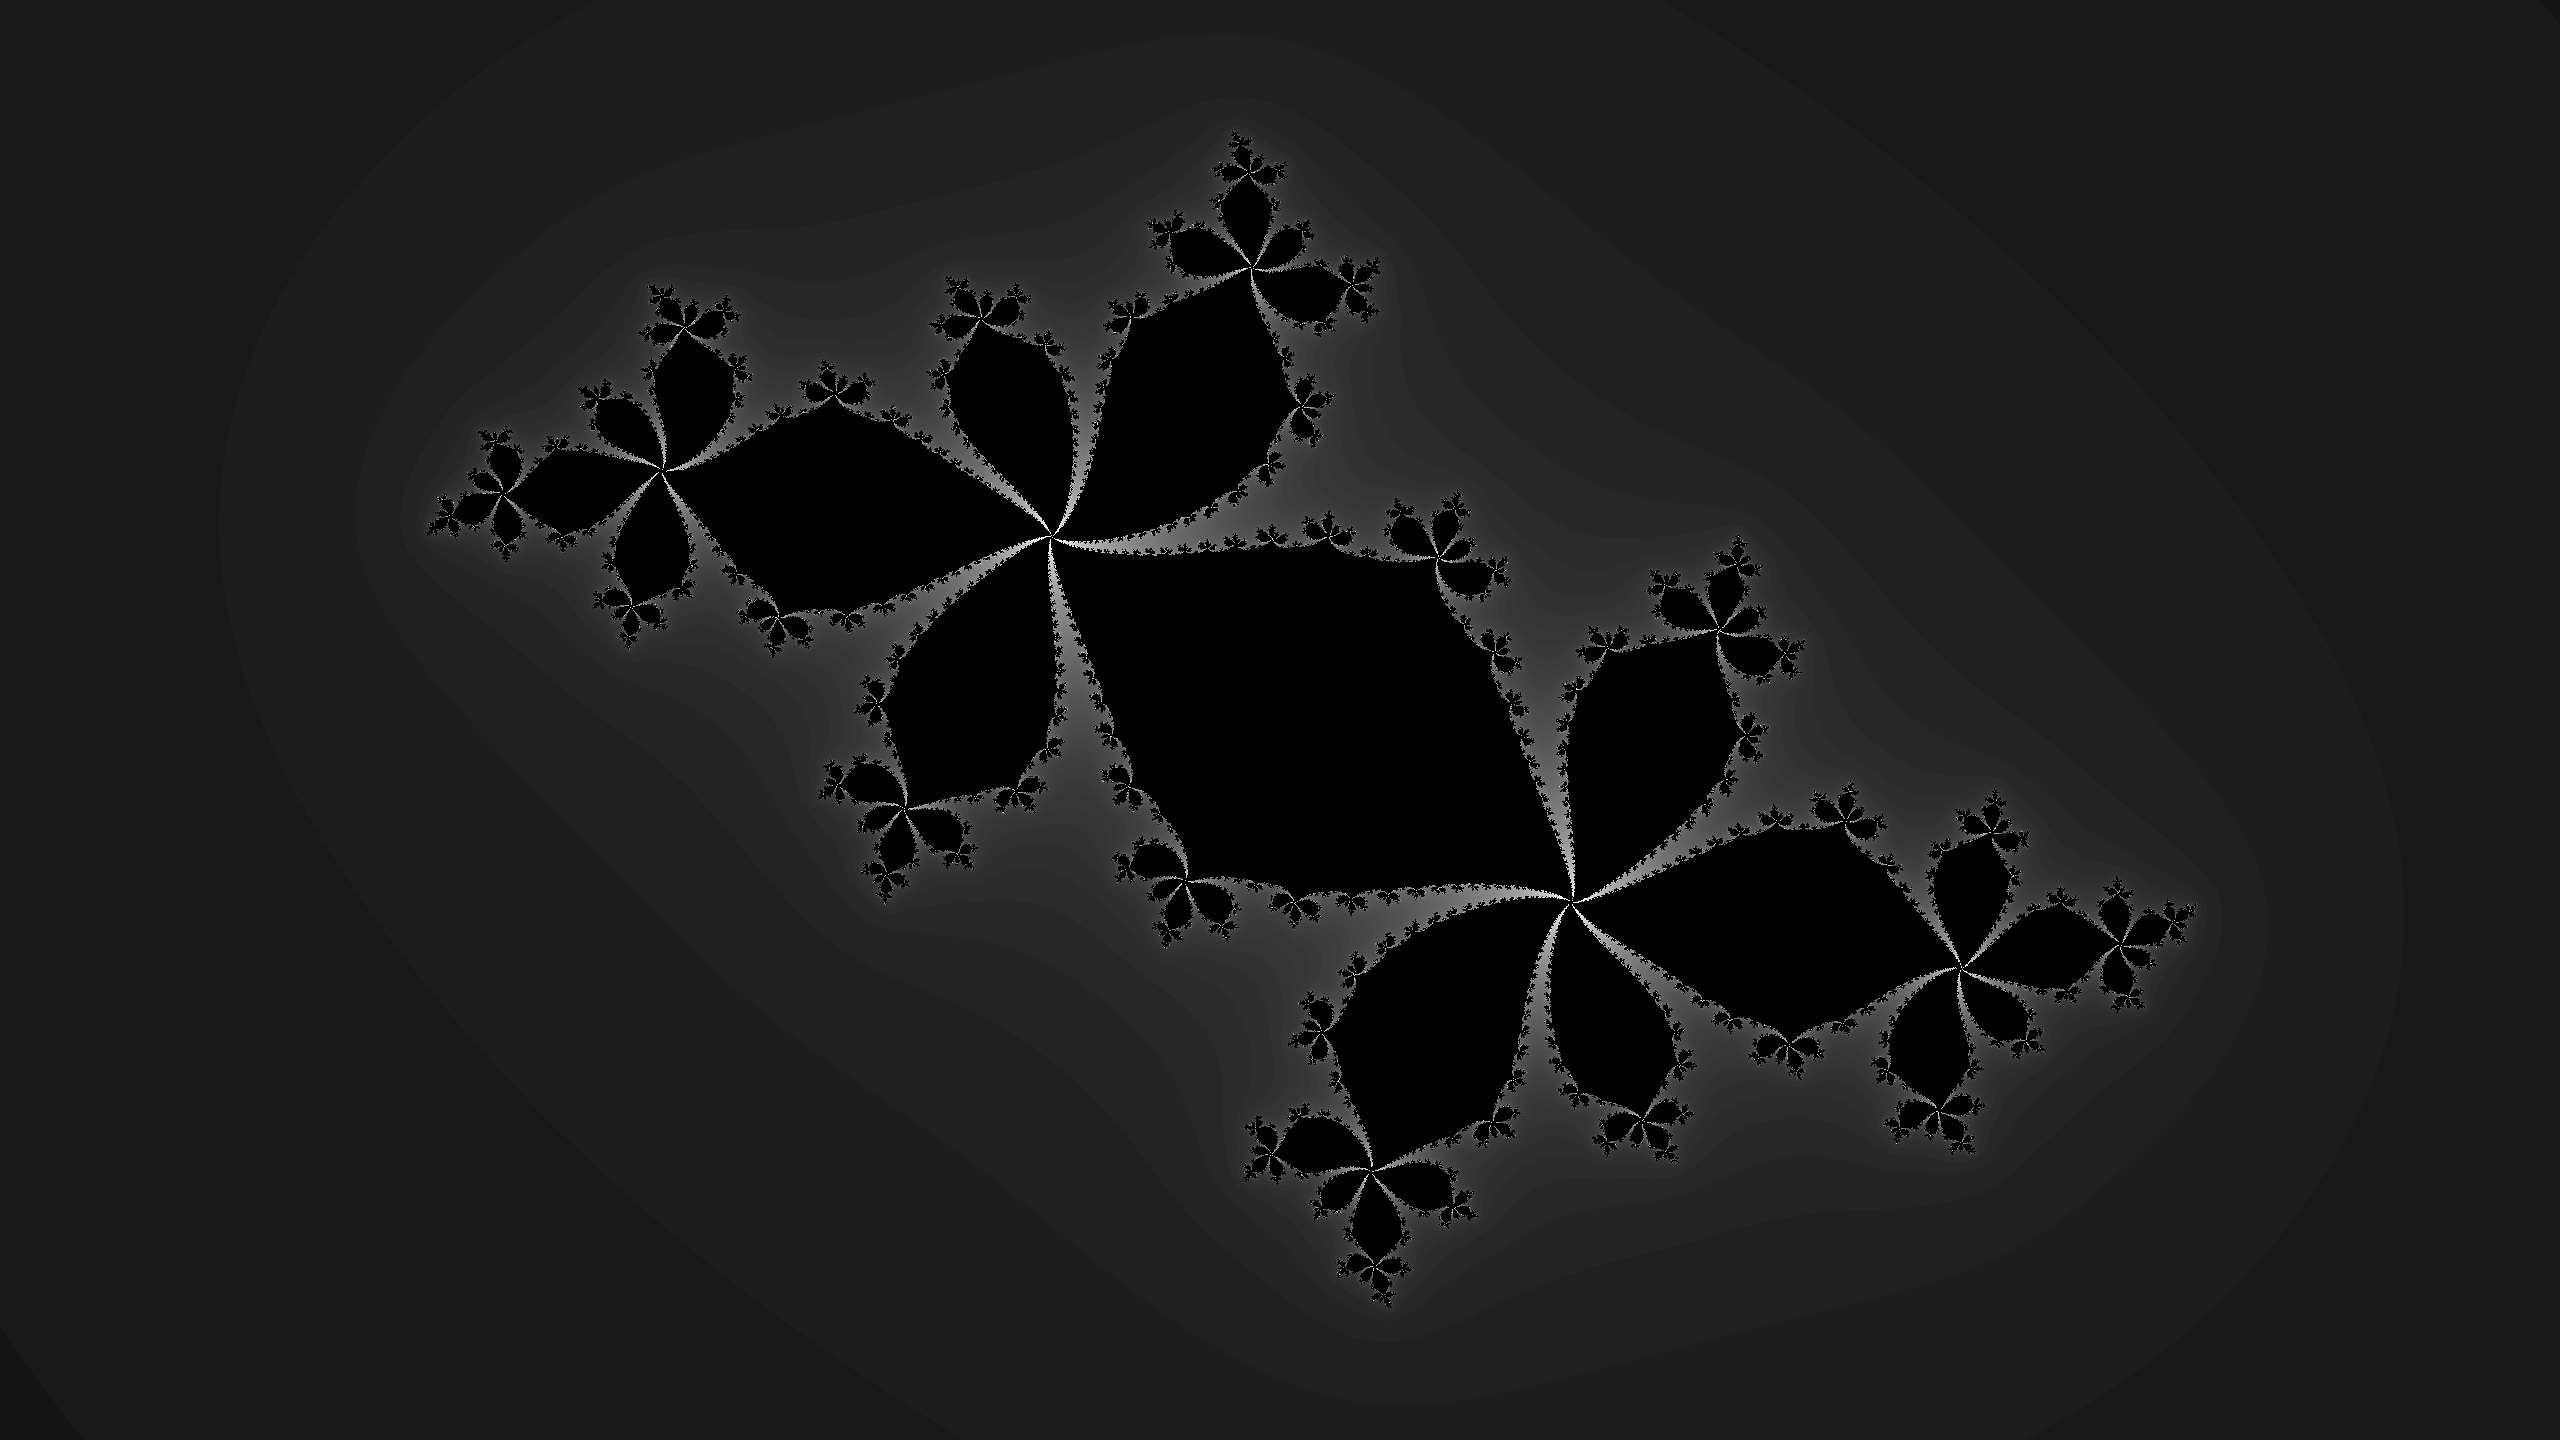
\includegraphics[width=\hsize]{julia/f.png}

\bigskip

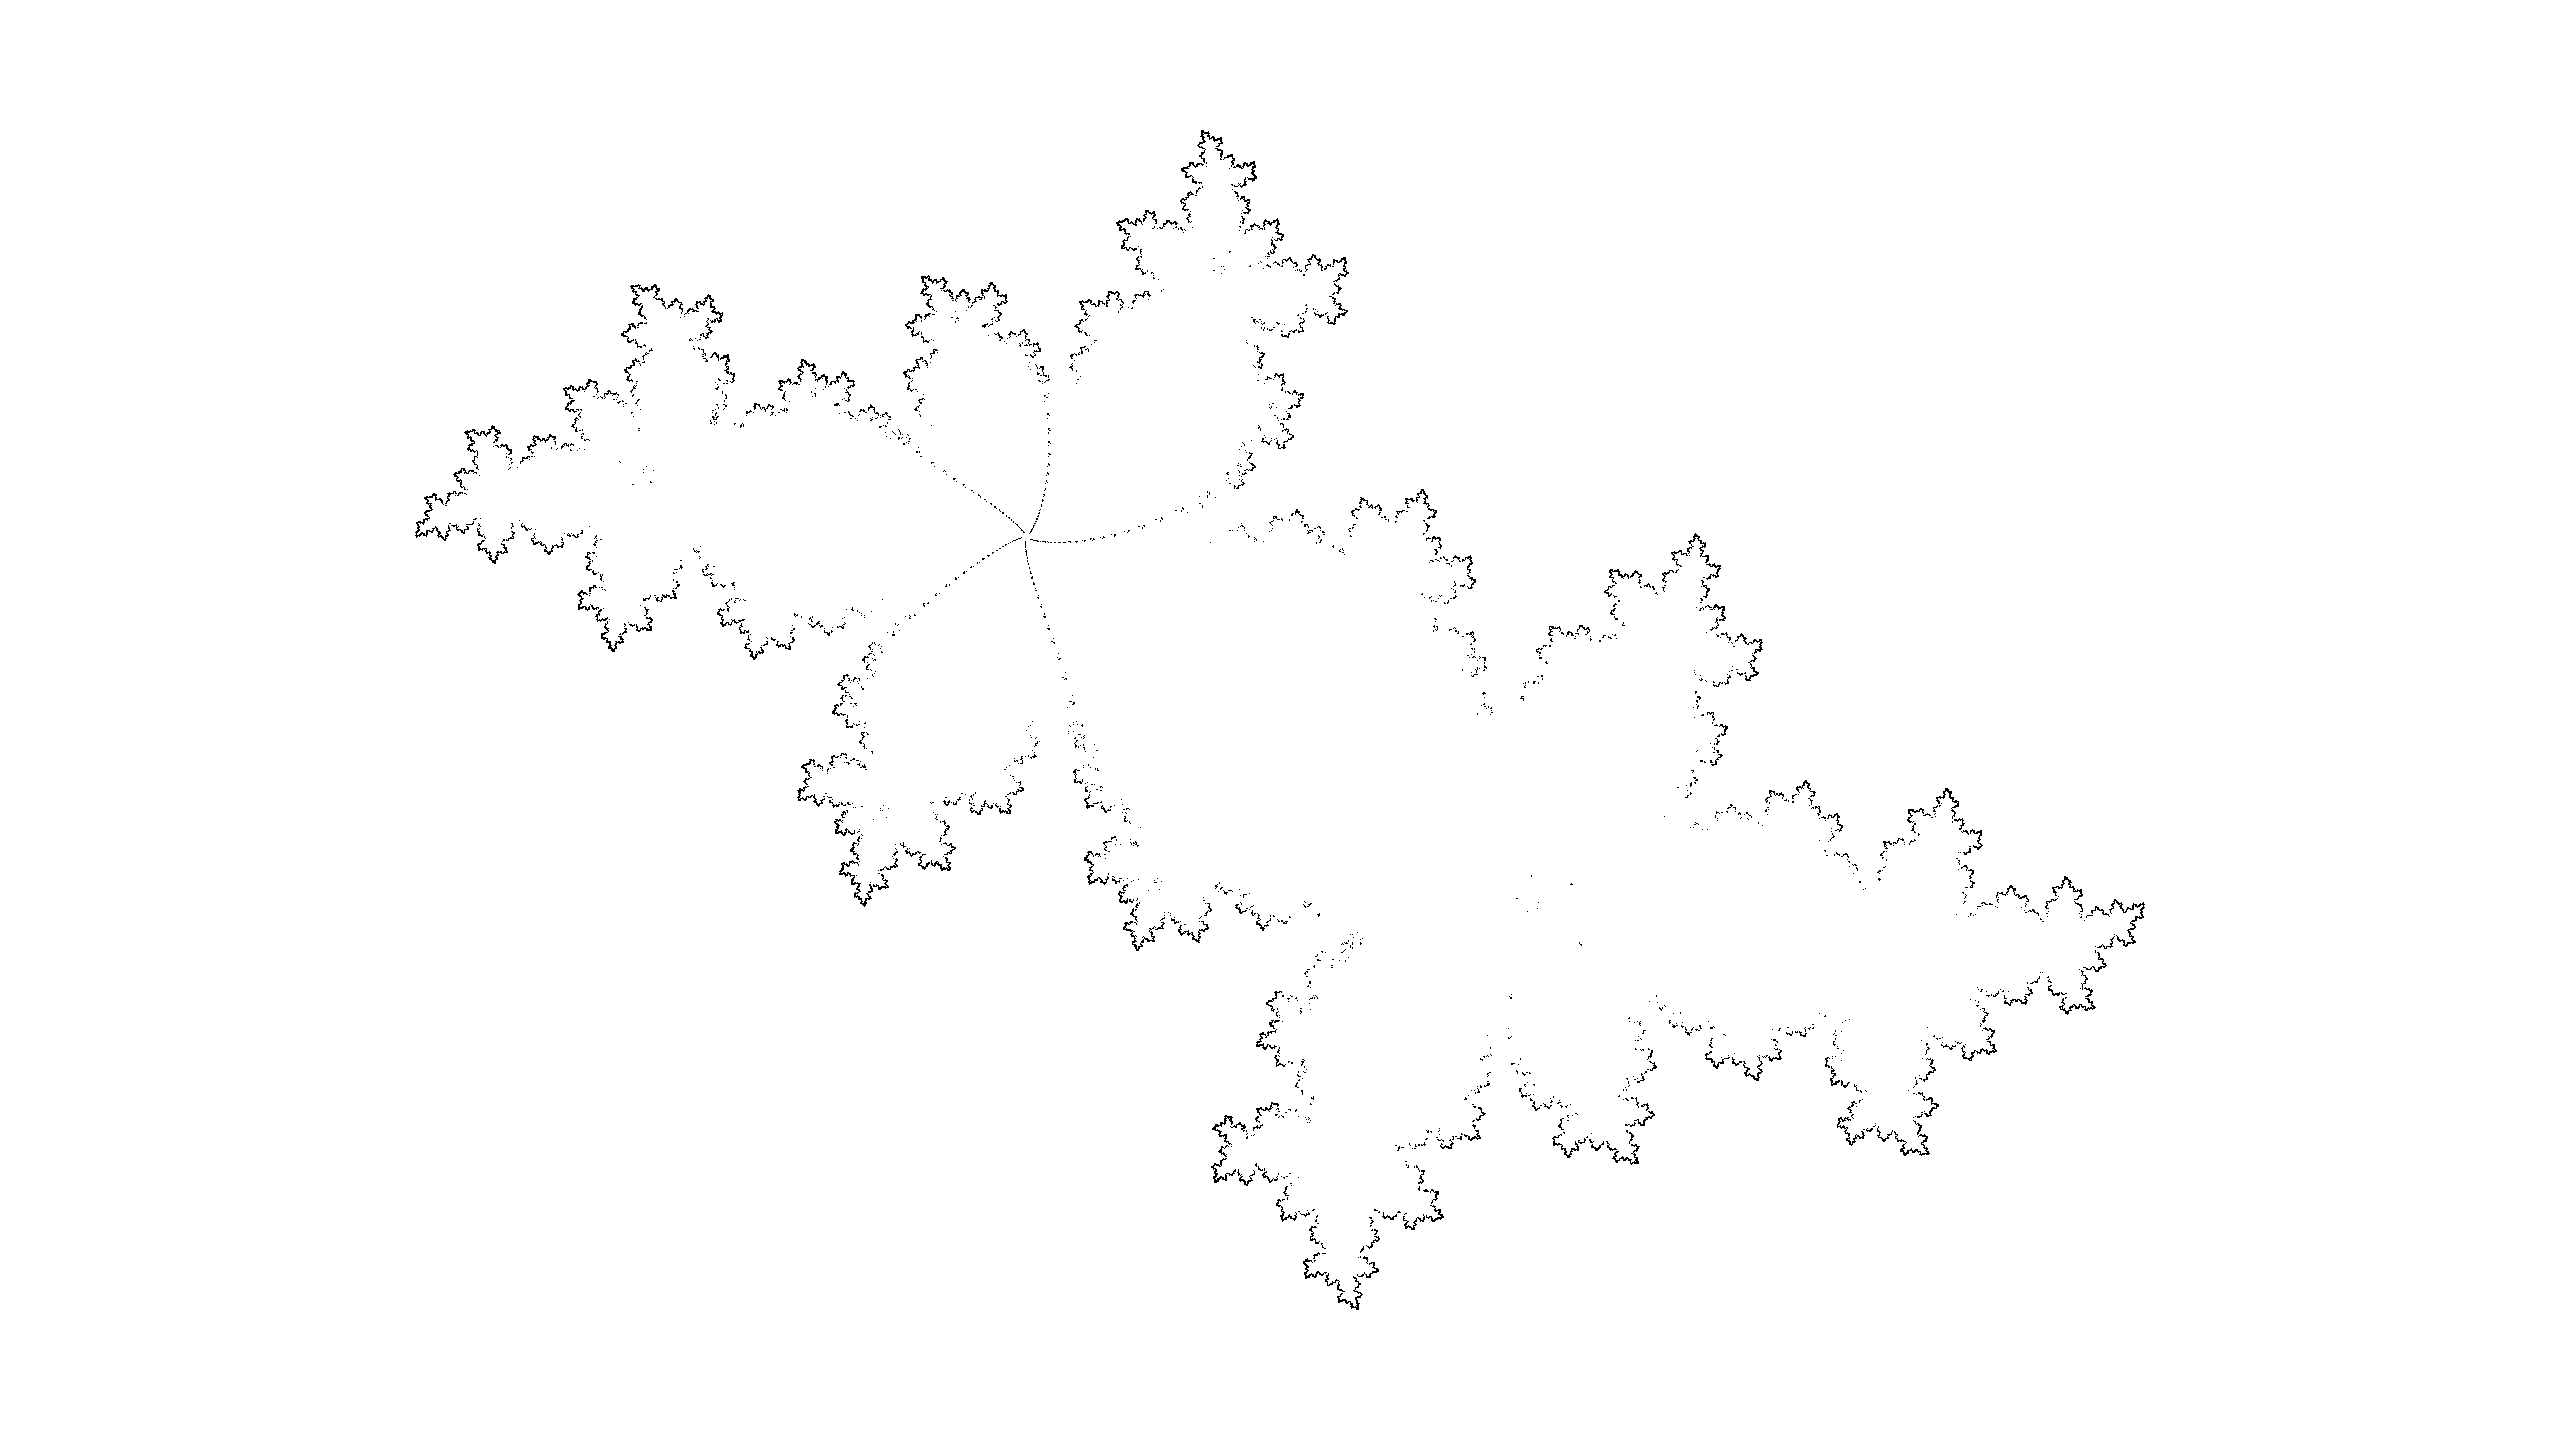
\includegraphics[width=\hsize]{julia/j-f.png}
\end{center}
\caption{Julia-Menge f"ur $c= -0.5+0.55i$}
\end{figure}

\begin{figure}
\begin{center}

\includegraphics[width=\hsize]{julia/g.png}

\bigskip

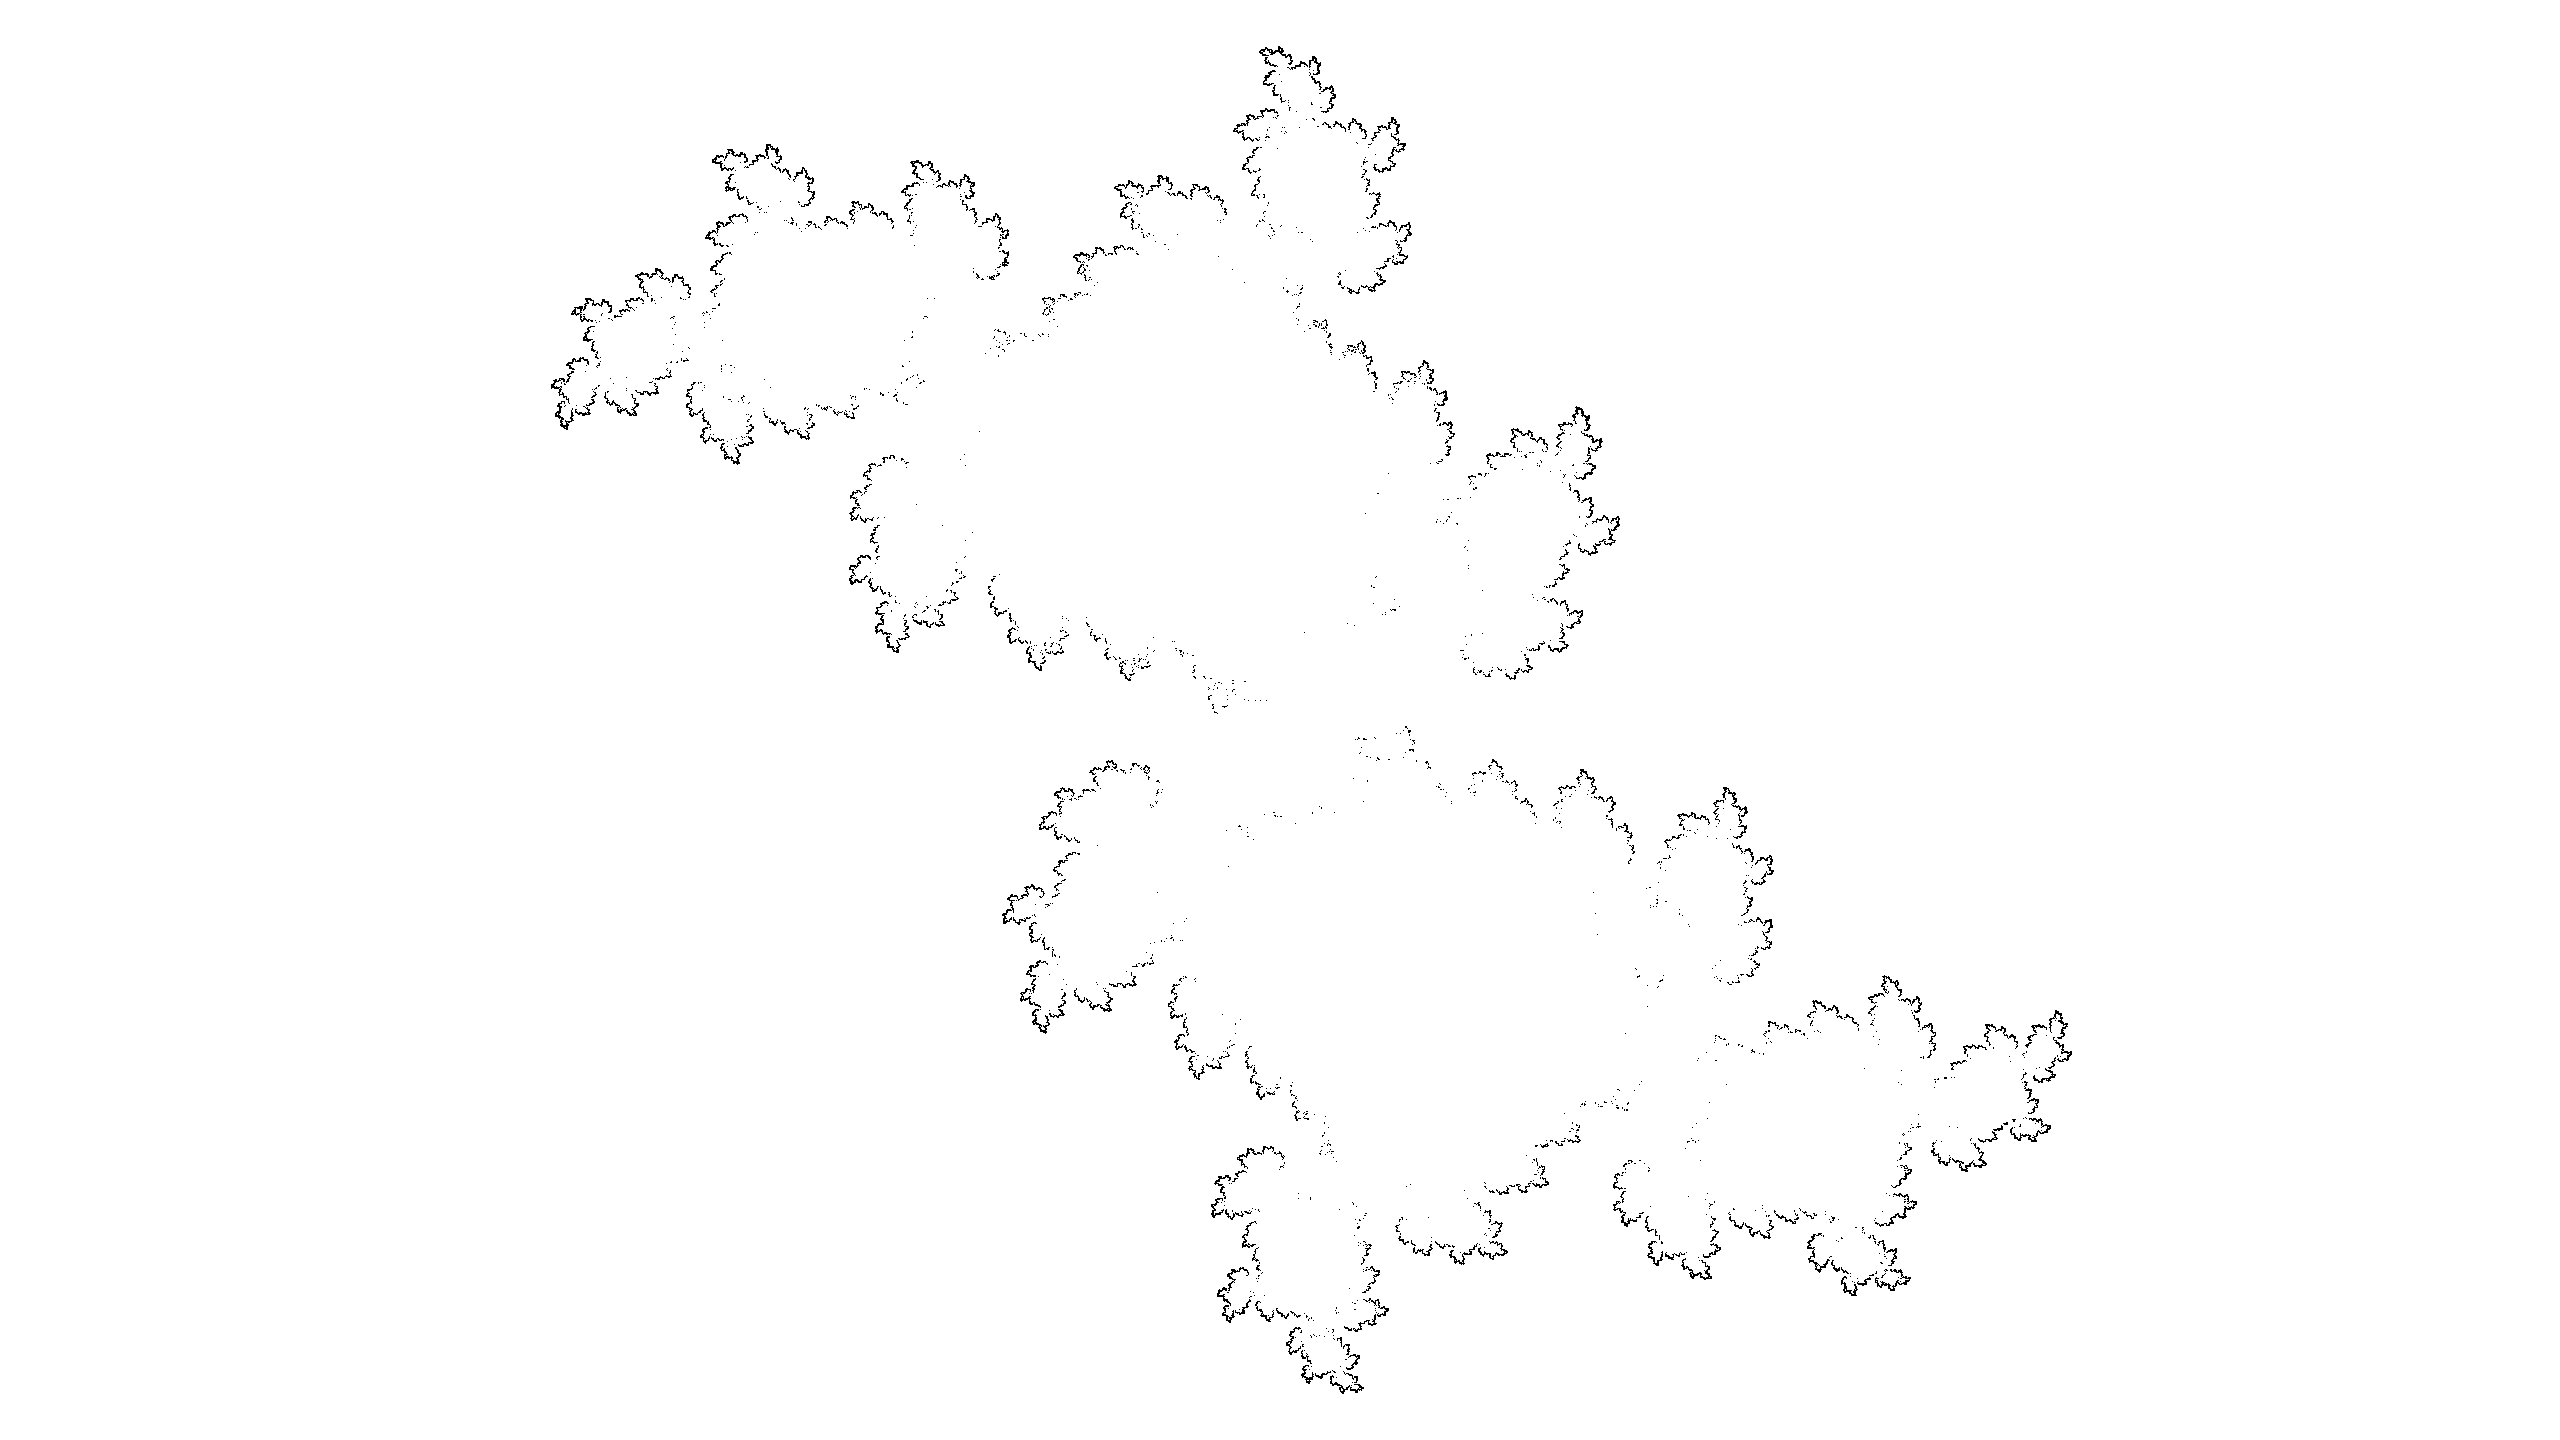
\includegraphics[width=\hsize]{julia/j-g.png}
\end{center}
\caption{Julia-Menge f"ur $c= 0.66i$}
\end{figure}

\begin{figure}
\begin{center}

\includegraphics[width=\hsize]{julia/h.png}

\bigskip

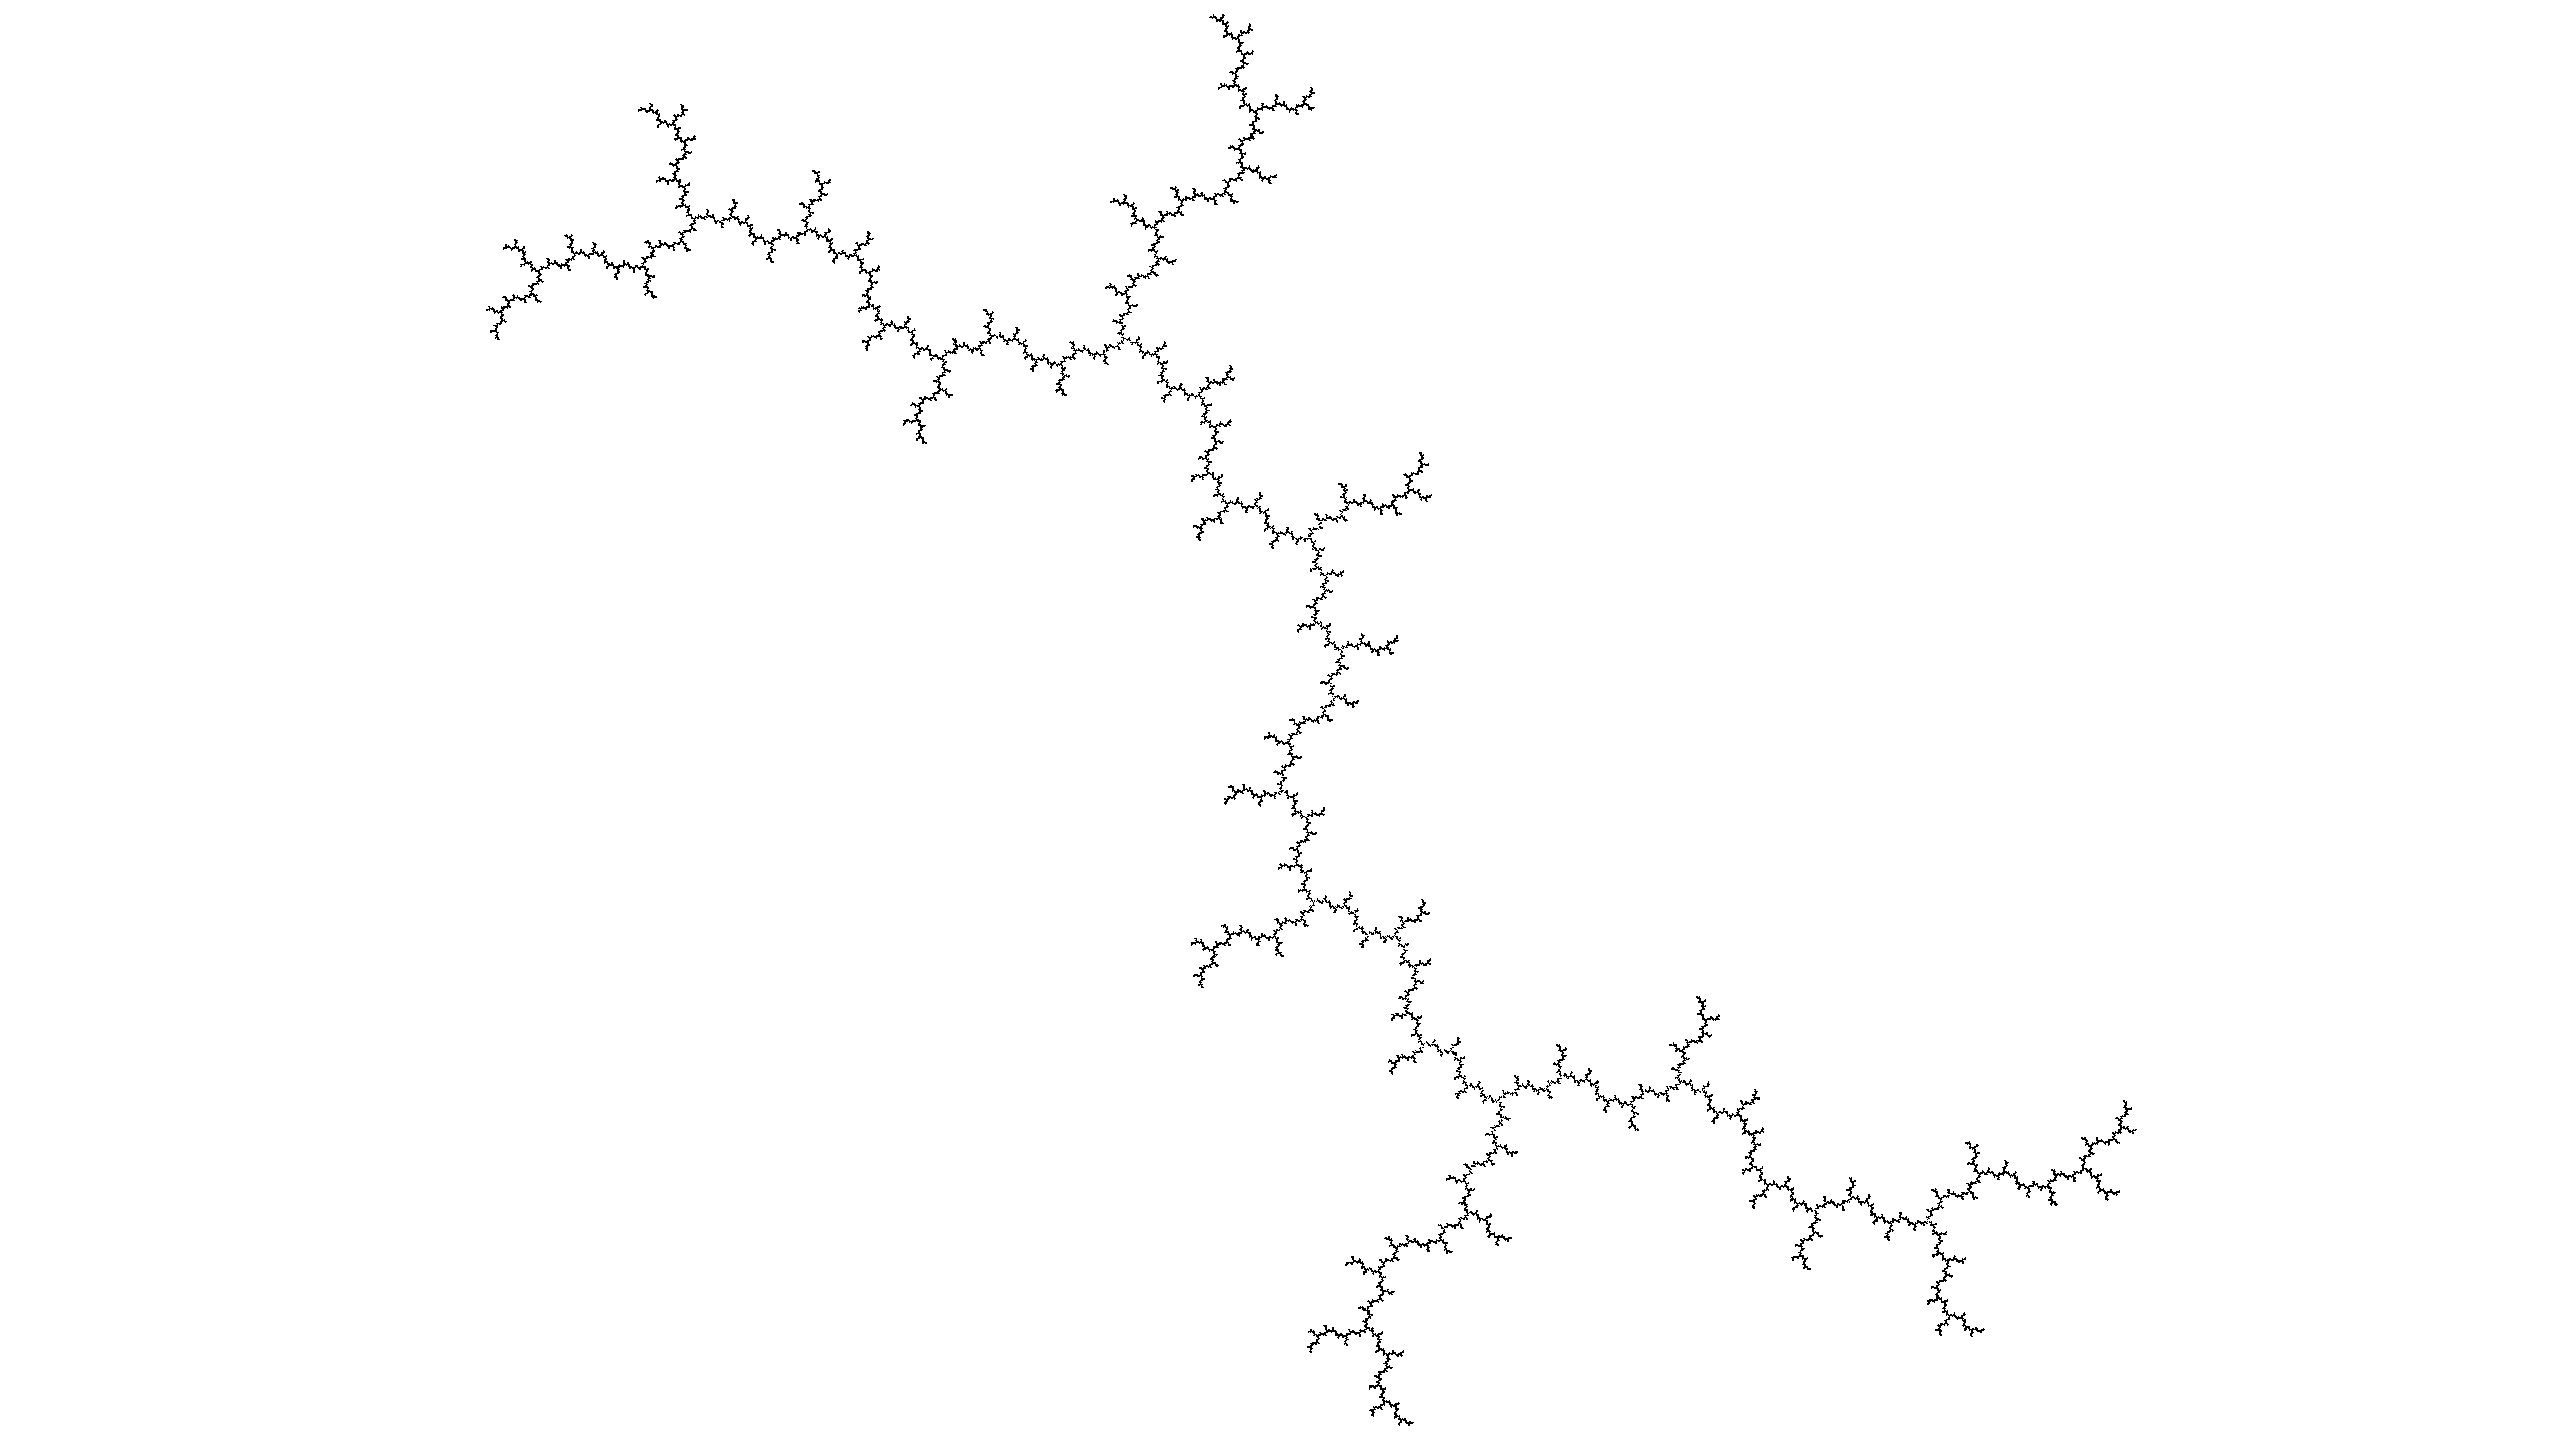
\includegraphics[width=\hsize]{julia/j-h.png}
\end{center}
\caption{Julia-Menge f"ur $c= -i$}
\end{figure}

\printbibliography[heading=subbibliography]
\end{refsection}
